% !TeX root = document.tex
% !TeX encoding = UTF-8 Unicode

\chapter{Results}%
\label{chp:results}

This chapter presents both simulations and experimental results that show the
technique working and compares it with dwell-time implementations.

For all simulations and experiments in this chapter, the controller is designed
to ensure null steady-state error for piecewise constant references at each mode
\(i\), and thus the integral action is applied over the tracking
error~\parencite{lopes.leite.ea:anti-windup}
%
\begin{equation}
  \label{eq:r-y-error}
  e(k) = r(k)-y(k),
\end{equation}
%
where \(r(k)\) is the desired output of the system. The proportional action
comes from the system's state deviation with respect to the equilibrium point.
Figure~\ref{fig:pi-controller-diagram} depicts the topology of the considered
controller.

\begin{figure}[!htb]
  \centering
  \resizebox{0.98\linewidth}{!}{\setlength{\unitlength}{4144sp}%
%
\begingroup\makeatletter\ifx\SetFigFont\undefined%
\gdef\SetFigFont#1#2#3#4#5{%
  \reset@font\fontsize{#1}{#2pt}%
  \fontfamily{#3}\fontseries{#4}\fontshape{#5}%
  \selectfont}%
\fi\endgroup%
\begin{picture}(10169,2767)(1914,-4943)
\thinlines
{\color[rgb]{0,0,0}\put(8866,-3301){\vector( 0, 1){630}}
}%
{\color[rgb]{0,0,0}\multiput(8551,-3211)(9.00000,0.00000){66}{\makebox(1.5875,11.1125){\tiny.}}
}%
{\color[rgb]{0,0,0}\multiput(9091,-2806)(-9.00000,0.00000){66}{\makebox(1.5875,11.1125){\tiny.}}
}%
{\color[rgb]{0,0,0}\put(8236,-2986){\vector( 1, 0){1260}}
}%
{\color[rgb]{0,0,0}\put(9377,-2809){\line(-1, 0){270}}
\put(9107,-2809){\line(-3,-2){591.923}}
\put(8522,-3214){\line(-1, 0){270}}
}%
\thicklines
{\color[rgb]{0,0,0}\put(8191,-3346){\framebox(1440,720){}}
}%
{\color[rgb]{0,0,0}\put(10576,-2356){\line(-1, 0){  2}}
\multiput(10565,-2358)(-10.00000,-2.00000){2}{\makebox(6.3500,9.5250){\small.}}
\multiput(10555,-2360)(-12.94120,-3.23530){2}{\makebox(6.3500,9.5250){\small.}}
\multiput(10542,-2363)(-8.00000,-2.00000){3}{\makebox(6.3500,9.5250){\small.}}
\multiput(10526,-2367)(-9.03845,-1.80769){3}{\makebox(6.3500,9.5250){\small.}}
\multiput(10508,-2371)(-10.94120,-2.73530){3}{\makebox(6.3500,9.5250){\small.}}
\multiput(10486,-2376)(-11.52940,-2.88235){3}{\makebox(6.3500,9.5250){\small.}}
\multiput(10463,-2382)(-8.31373,-2.07843){4}{\makebox(6.3500,9.5250){\small.}}
\multiput(10438,-2388)(-8.60000,-2.86667){4}{\makebox(6.3500,9.5250){\small.}}
\multiput(10412,-2396)(-8.60000,-2.86667){4}{\makebox(6.3500,9.5250){\small.}}
\multiput(10386,-2404)(-9.00000,-3.00000){4}{\makebox(6.3500,9.5250){\small.}}
\multiput(10359,-2413)(-8.90803,-3.56321){4}{\makebox(6.3500,9.5250){\small.}}
\multiput(10332,-2423)(-9.31033,-3.72413){4}{\makebox(6.3500,9.5250){\small.}}
\multiput(10304,-2434)(-9.71263,-3.88505){4}{\makebox(6.3500,9.5250){\small.}}
\multiput(10275,-2446)(-7.20000,-3.60000){5}{\makebox(6.3500,9.5250){\small.}}
\multiput(10246,-2460)(-7.60000,-3.80000){5}{\makebox(6.3500,9.5250){\small.}}
\multiput(10216,-2476)(-7.50000,-4.50000){5}{\makebox(6.3500,9.5250){\small.}}
\multiput(10186,-2494)(-7.67307,-5.11538){5}{\makebox(6.3500,9.5250){\small.}}
\multiput(10155,-2514)(-7.28000,-5.46000){5}{\makebox(6.3500,9.5250){\small.}}
\multiput(10126,-2536)(-6.64918,-5.54098){6}{\makebox(6.3500,9.5250){\small.}}
\multiput(10093,-2564)(-5.70000,-5.70000){6}{\makebox(6.3500,9.5250){\small.}}
\multiput(10064,-2592)(-5.67622,-6.81147){5}{\makebox(6.3500,9.5250){\small.}}
\multiput(10041,-2619)(-4.92000,-6.56000){5}{\makebox(6.3500,9.5250){\small.}}
\multiput(10021,-2645)(-5.48717,-8.23075){4}{\makebox(6.3500,9.5250){\small.}}
\multiput(10005,-2670)(-4.52940,-7.54900){4}{\makebox(6.3500,9.5250){\small.}}
\multiput(9992,-2693)(-3.80000,-7.60000){4}{\makebox(6.3500,9.5250){\small.}}
\multiput(9981,-2716)(-3.70000,-11.10000){3}{\makebox(6.3500,9.5250){\small.}}
\multiput(9973,-2738)(-3.65000,-10.95000){3}{\makebox(6.3500,9.5250){\small.}}
\multiput(9966,-2760)(-3.30000,-9.90000){3}{\makebox(6.3500,9.5250){\small.}}
\multiput(9960,-2780)(-1.80770,-9.03850){3}{\makebox(6.3500,9.5250){\small.}}
\multiput(9956,-2798)(-2.00000,-8.00000){3}{\makebox(6.3500,9.5250){\small.}}
\multiput(9952,-2814)(-2.32430,-13.94580){2}{\makebox(6.3500,9.5250){\small.}}
\multiput(9950,-2828)(-2.82355,-11.29420){3}{\makebox(6.3500,9.5250){\small.}}
\put(9944,-2851){\vector(-1,-4){0}}
}%
{\color[rgb]{0,0,0}\put(4264,-4030){\framebox(879,603){}}
}%
{\color[rgb]{0,0,0}\put(8201,-4291){\framebox(1105,720){}}
}%
{\color[rgb]{0,0,0}\thinlines
\put(2566,-3031){\circle{484}}
}%
{\color[rgb]{0,0,0}\put(3781,-3031){\circle{484}}
}%
{\color[rgb]{0,0,0}\put(7381,-2941){\circle{484}}
}%
\thicklines
{\color[rgb]{0,0,0}\put(1936,-3076){\vector( 1, 0){405}}
}%
{\color[rgb]{0,0,0}\put(2836,-3076){\vector( 1, 0){720}}
}%
{\color[rgb]{0,0,0}\put(4231,-3706){\line(-1, 0){450}}
\put(3781,-3706){\vector( 0, 1){450}}
}%
{\color[rgb]{0,0,0}\put(7606,-2986){\vector( 1, 0){585}}
}%
{\color[rgb]{0,0,0}\put(9631,-2986){\vector( 1, 0){450}}
}%
{\color[rgb]{0,0,0}\put(6841,-2986){\vector( 1, 0){315}}
}%
{\color[rgb]{0,0,0}\put(5401,-3031){\line( 0,-1){675}}
\put(5401,-3706){\vector(-1, 0){270}}
}%
{\color[rgb]{0,0,0}\put(5716,-3391){\framebox(1125,675){}}
}%
{\color[rgb]{0,0,0}\put(4051,-3031){\vector( 1, 0){1665}}
}%
{\color[rgb]{0,0,0}\put(10036,-3346){\framebox(1665,720){}}
}%
{\color[rgb]{0,0,0}\put(8191,-3976){\line(-1, 0){810}}
\put(7381,-3976){\vector( 0, 1){810}}
}%
{\color[rgb]{0,0,0}\put(11701,-2986){\line( 1, 0){360}}
\put(12061,-2986){\line( 0,-1){1935}}
\put(12061,-4921){\line(-1, 0){9495}}
\put(2566,-4921){\vector( 0, 1){1665}}
}%
{\color[rgb]{0,0,1}\put(3286,-4741){\dashbox{114}(3645,2205){}}
}%
{\color[rgb]{0,0,0}\put(10036,-4336){\framebox(1665,720){}}
}%
{\color[rgb]{0,0,0}\put(12061,-4156){\vector(-1, 0){405}}
}%
{\color[rgb]{0,0,0}\put(9811,-2986){\line( 0,-1){495}}
\put(9811,-3481){\line( 1, 0){2115}}
\put(11926,-3481){\line( 0,-1){360}}
\put(11926,-3841){\vector(-1, 0){270}}
}%
{\color[rgb]{0,0,0}\put(10036,-3976){\vector(-1, 0){765}}
}%
{\color[rgb]{.69,0,0}\put(7156,-4741){\dashbox{57}(2520,1305){}}
}%
\thinlines
{\color[rgb]{0,0,0}\multiput(6311,-3661)(12.00000,3.00000){2}{\makebox(1.5875,11.1125){\tiny.}}
\multiput(6323,-3658)(8.40000,2.80000){3}{\makebox(1.5875,11.1125){\tiny.}}
\multiput(6340,-3653)(7.90000,2.63333){4}{\makebox(1.5875,11.1125){\tiny.}}
\multiput(6364,-3646)(9.60000,3.20000){4}{\makebox(1.5875,11.1125){\tiny.}}
\multiput(6393,-3637)(8.40000,2.80000){5}{\makebox(1.5875,11.1125){\tiny.}}
\multiput(6427,-3627)(9.00000,3.00000){5}{\makebox(1.5875,11.1125){\tiny.}}
\multiput(6463,-3615)(7.74000,2.58000){6}{\makebox(1.5875,11.1125){\tiny.}}
\multiput(6502,-3603)(7.92000,2.64000){6}{\makebox(1.5875,11.1125){\tiny.}}
\multiput(6542,-3591)(7.80000,2.60000){6}{\makebox(1.5875,11.1125){\tiny.}}
\multiput(6581,-3578)(9.30000,3.10000){5}{\makebox(1.5875,11.1125){\tiny.}}
\multiput(6618,-3565)(9.00000,3.00000){5}{\makebox(1.5875,11.1125){\tiny.}}
\multiput(6654,-3553)(8.32500,2.77500){5}{\makebox(1.5875,11.1125){\tiny.}}
\multiput(6687,-3541)(7.50000,3.00000){5}{\makebox(1.5875,11.1125){\tiny.}}
\multiput(6717,-3529)(9.71263,3.88505){4}{\makebox(1.5875,11.1125){\tiny.}}
\multiput(6746,-3517)(8.44827,3.37931){4}{\makebox(1.5875,11.1125){\tiny.}}
\multiput(6771,-3506)(7.86667,3.93333){4}{\makebox(1.5875,11.1125){\tiny.}}
\multiput(6795,-3495)(10.60000,5.30000){3}{\makebox(1.5875,11.1125){\tiny.}}
\multiput(6816,-3484)(9.77940,5.86764){3}{\makebox(1.5875,11.1125){\tiny.}}
\multiput(6836,-3473)(9.04410,5.42646){3}{\makebox(1.5875,11.1125){\tiny.}}
\multiput(6854,-3462)(8.42310,5.61540){3}{\makebox(1.5875,11.1125){\tiny.}}
\multiput(6871,-3451)(8.00000,6.00000){3}{\makebox(1.5875,11.1125){\tiny.}}
\multiput(6887,-3439)(9.00000,7.50000){3}{\makebox(1.5875,11.1125){\tiny.}}
\multiput(6905,-3424)(8.70490,7.25408){3}{\makebox(1.5875,11.1125){\tiny.}}
\multiput(6922,-3409)(8.25000,8.25000){3}{\makebox(1.5875,11.1125){\tiny.}}
\multiput(6938,-3392)(7.50000,9.00000){3}{\makebox(1.5875,11.1125){\tiny.}}
\multiput(6953,-3374)(4.51283,6.76925){4}{\makebox(1.5875,11.1125){\tiny.}}
\multiput(6967,-3354)(4.82050,7.23075){4}{\makebox(1.5875,11.1125){\tiny.}}
\multiput(6981,-3332)(4.76470,7.94117){4}{\makebox(1.5875,11.1125){\tiny.}}
\multiput(6995,-3308)(5.14707,8.57844){4}{\makebox(1.5875,11.1125){\tiny.}}
\multiput(7010,-3282)(3.60000,7.20000){5}{\makebox(1.5875,11.1125){\tiny.}}
\multiput(7024,-3253)(3.80000,7.60000){5}{\makebox(1.5875,11.1125){\tiny.}}
\multiput(7038,-3222)(3.12070,7.80175){5}{\makebox(1.5875,11.1125){\tiny.}}
\multiput(7051,-3191)(3.24138,8.10344){5}{\makebox(1.5875,11.1125){\tiny.}}
\multiput(7065,-3159)(3.08620,7.71550){5}{\makebox(1.5875,11.1125){\tiny.}}
\multiput(7077,-3128)(3.72413,9.31033){4}{\makebox(1.5875,11.1125){\tiny.}}
\multiput(7088,-3100)(3.17240,7.93100){4}{\makebox(1.5875,11.1125){\tiny.}}
\multiput(7097,-3076)(2.82000,8.46000){6}{\makebox(1.5875,11.1125){\tiny.}}
\put(7111,-3034){\vector( 1, 3){0}}
}%
\put(9226,-3211){\makebox(0,0)[rb]{\smash{{\SetFigFont{12}{14.4}{\rmdefault}{\mddefault}{\updefault}{\color[rgb]{0,0,0}\(\underbar{u}\)}%
}}}}
\put(8461,-2896){\makebox(0,0)[rb]{\smash{{\SetFigFont{12}{14.4}{\rmdefault}{\mddefault}{\updefault}{\color[rgb]{0,0,0}\(\bar{u}\)}%
}}}}
\put(10621,-2311){\makebox(0,0)[rb]{\smash{{\SetFigFont{12}{14.4}{\rmdefault}{\mddefault}{\updefault}{\color[rgb]{0,0,0}\(\textrm{sat}(u(k))\)}%
}}}}
\put(4622,-3746){\makebox(0,0)[lb]{\smash{{\SetFigFont{9}{10.8}{\rmdefault}{\mddefault}{\updefault}{\color[rgb]{0,0,0}\(z^{-1}\)}%
}}}}
\put(8643,-3976){\makebox(0,0)[lb]{\smash{{\SetFigFont{14}{16.8}{\rmdefault}{\mddefault}{\updefault}{\color[rgb]{0,0,0}\(K\)}%
}}}}
\put(2341,-3481){\makebox(0,0)[lb]{\smash{{\SetFigFont{12}{14.4}{\rmdefault}{\mddefault}{\updefault}{\color[rgb]{0,0,0}-}%
}}}}
\put(3376,-2896){\makebox(0,0)[lb]{\smash{{\SetFigFont{12}{14.4}{\rmdefault}{\mddefault}{\updefault}{\color[rgb]{0,0,0}+}%
}}}}
\put(3556,-3436){\makebox(0,0)[lb]{\smash{{\SetFigFont{12}{14.4}{\rmdefault}{\mddefault}{\updefault}{\color[rgb]{0,0,0}+}%
}}}}
\put(2026,-3256){\makebox(0,0)[lb]{\smash{{\SetFigFont{12}{14.4}{\rmdefault}{\mddefault}{\updefault}{\color[rgb]{0,0,0}+}%
}}}}
\put(1981,-2941){\makebox(0,0)[lb]{\smash{{\SetFigFont{12}{14.4}{\rmdefault}{\mddefault}{\updefault}{\color[rgb]{0,0,0}\(r(k)\)}%
}}}}
\put(2791,-3976){\makebox(0,0)[lb]{\smash{{\SetFigFont{12}{14.4}{\rmdefault}{\mddefault}{\updefault}{\color[rgb]{0,0,0}\(y(k)\)}%
}}}}
\put(7021,-2851){\makebox(0,0)[lb]{\smash{{\SetFigFont{12}{14.4}{\rmdefault}{\mddefault}{\updefault}{\color[rgb]{0,0,0}+}%
}}}}
\put(7516,-3661){\makebox(0,0)[lb]{\smash{{\SetFigFont{12}{14.4}{\rmdefault}{\mddefault}{\updefault}{\color[rgb]{0,0,0}\(u_p(k)\)}%
}}}}
\put(7786,-3166){\makebox(0,0)[lb]{\smash{{\SetFigFont{12}{14.4}{\rmdefault}{\mddefault}{\updefault}{\color[rgb]{0,0,0}\(u(k)\)}%
}}}}
\put(6346,-3886){\makebox(0,0)[lb]{\smash{{\SetFigFont{12}{14.4}{\rmdefault}{\mddefault}{\updefault}{\color[rgb]{0,0,0}\(u_i(k)\)}%
}}}}
\put(3501,-3931){\makebox(0,0)[lb]{\smash{{\SetFigFont{12}{14.4}{\rmdefault}{\mddefault}{\updefault}{\color[rgb]{0,0,0}\(v(k-1)\)}%
}}}}
\put(6346,-3076){\makebox(0,0)[lb]{\smash{{\SetFigFont{8}{9.6}{\rmdefault}{\mddefault}{\updefault}{\color[rgb]{0,0,0}\(K_i\)}%
}}}}
\put(10801,-2986){\makebox(0,0)[lb]{\smash{{\SetFigFont{12}{14.4}{\rmdefault}{\mddefault}{\updefault}{\color[rgb]{0,0,0}sys}%
}}}}
\put(4681,-2896){\makebox(0,0)[lb]{\smash{{\SetFigFont{12}{14.4}{\rmdefault}{\mddefault}{\updefault}{\color[rgb]{0,0,0}\(v(k)\)}%
}}}}
\put(2861,-2941){\makebox(0,0)[lb]{\smash{{\SetFigFont{12}{14.4}{\rmdefault}{\mddefault}{\updefault}{\color[rgb]{0,0,0}\(e(k)\)}%
}}}}
\put(7156,-3391){\makebox(0,0)[lb]{\smash{{\SetFigFont{12}{14.4}{\rmdefault}{\mddefault}{\updefault}{\color[rgb]{0,0,0}+}%
}}}}
\put(7291,-4516){\makebox(0,0)[lb]{\smash{{\SetFigFont{12}{14.4}{\rmdefault}{\mddefault}{\updefault}{\color[rgb]{.69,0,0}Proportional Action}%
}}}}
\put(3466,-4516){\makebox(0,0)[lb]{\smash{{\SetFigFont{12}{14.4}{\rmdefault}{\mddefault}{\updefault}{\color[rgb]{0,0,1}Integral Action}%
}}}}
\put(10756,-4021){\makebox(0,0)[lb]{\smash{{\SetFigFont{12}{14.4}{\rmdefault}{\mddefault}{\updefault}{\color[rgb]{0,0,0}obs}%
}}}}
\put(9511,-3886){\makebox(0,0)[lb]{\smash{{\SetFigFont{12}{14.4}{\rmdefault}{\mddefault}{\updefault}{\color[rgb]{0,0,0}\(x(k)\)}%
}}}}
\end{picture}%
}
  \caption[PI-like controller.]{PI-like controller. The states are fedback
    proportionally and the output error is integrated to obtain reference
    tracking.}%
  \label{fig:pi-controller-diagram}
\end{figure}

By defining an augmented state vector
\[
  \xi(k)=\begin{bmatrix}{x(k)}^\top &v{(k)}^\top\end{bmatrix}^\top,
\]
where \(v(k)\in\mathbb{R}^{n_u}\) is the vector of added integrators, the
closed-loop system shown in Figure~\ref{fig:pi-controller-diagram} can be
rewritten as

\begin{equation}
  \label{eq:augmented-system}
  \begin{split}
    \xi(k+1) &= \mathcal{A}_i\xi(k)+\mathcal{B}_{i}u(k), \\
    y_{k}    &= \mathcal{C}_i\xi(k)+\mathcal{D}_{i}u(k),
  \end{split}
\end{equation}

where \(\mathcal{A}_i=\begin{bmatrix}A_i & \textbf{0} \\-C_{i}&\textbf{I}
\end{bmatrix} \), \(\mathcal{B}_i=\begin{bmatrix}B_i\\D_i\end{bmatrix}\),
\(\mathcal{C}_i=\begin{bmatrix} C_i & \textbf{0} \end{bmatrix}\),
\(\mathcal{D}_i=\begin{bmatrix}\mathcal{D}_i^\top&\textbf{0}\end{bmatrix}^\top\).

The design of each controller gain \(K_i\in\mathbb{R}^{n_u\times{}(n+p)}\) may use
tandard LMI based techniques, such as, for instance, pole
placement~\parencite{yu:lmis}, LPV design~\parencite{briat:linear}, or robust
control~\parencite{boyd.ghaoui.ea:linear}. The exponential stability and
saturation LMI's described below were used.

Note that the constrained output can also be expressed in terms of the augmented
state \(\xi(k)\), taking into account the state of the integrator, i.e., \(c(k)\)
in~\eqref{eq:state-space} can be given by
%
\begin{equation}
  \label{eq:constrained-output}
  c(k) = \mathcal{E}_i\xi(k) + \mathcal{F}_i u(k),
\end{equation}
%
with the mode-dependent matrices \(\mathcal{E}_i\) and \(\mathcal{F}_i\) with
adequate dimensions.

There are various ways to measure stability, with the asymptotic stability being
the most common. However, other definitions might yield better results. One of
such stability criteria is exponential stability, which guarantees fast
convergence to the origin. A system is said to be exponentially stable if its
states decay is upper-bounded by an exponential~\parencite{hespanha:linear}:
%
\begin{equation}
  \norm{x(t)} \le{} Ce^{-\lambda{}(t-t_{0})}\norm{x(0)}.
\end{equation}
%
Squaring both sides of the equation and expanding the norms we get
%
\begin{equation}
  x(t)^{T}x(t) \le{} C^{2}e^{-2\lambda{}(t-t_{0})}x(0)^{T}x(0).
\end{equation}
%
Using Taylor's series approximation to discretize the equation with \(C=1\) and
letting the constant \(\lambda{}\) absorb the constant \(2\) yields
%
\begin{equation}
  x(k+1)^{T}x(k+1) \le{} (1-\lambda{}) x(k)^{T}x(k).
\end{equation}
%
Inserting the matrix \(P\) between both vectors does not affect the innequality.
Replacing \(x(k+1)=(A+BK)x(k)\) results in
%
\begin{equation}
  x(k)^{T}[(A+BK)^{T}P(A+BK)-(I-\lambda{}I)P]x(k) \prec \mathbf{0}.
\end{equation}
%
Applying the Schur complement we obtain
%
\begin{equation}
  \begin{bmatrix}
    (I-\lambda{}I)P & (A+BK)^{T}P \\
    P(A+BK)         & P
  \end{bmatrix} \succ \mathbf{0}
\end{equation}
%
Pre- and post-multiplying by
\(\left[\begin{smallmatrix} P^{-1} & 0 \\ 0 & P^{-1}
  \end{smallmatrix}\right]\) and making \(W=P^{-1}\) and \(Z=KP^{-1}\), we
obtain our LMI, which can be used with the following optimization procedure:
%
\begin{align}
  \label{eq:roa-opt}
  \min_{W,Z}     & \texttt{ Trace}(W) \nonumber                 \\
  \textrm{s. t.} & \begin{bmatrix}
    W(I-\lambda{}I) & (AW+BZ)^{T} \\
    AW+BZ           & W
  \end{bmatrix} \succ \mathbf{0}.
\end{align}

Considering~\eqref{eq:augmented-system} under input saturation, even though the
input constraints are usually included in the set \(\mathcal{C}\) and are
handled by the optimization machinery, at this point, we explicitly consider
them, by using a saturating allowance
approach~\parencite{tarbouriech.garcia.ea:stability}. In such a case, we assume
decentralized saturation function, \(\sat{u(k)}\), instead of \(u(k)\) as the
input signal in~\eqref{eq:augmented-system}, where \(\bar{u}\) is the saturation
value and
%
\[
  \sat{u} = \mbox{\textrm{sign}}(U_{\ell})\min\{|u_{(\ell)}|,\bar{u}_{(\ell)}\}, \quad \ell = 1,\ldots, m,
\] where \(u_{(\ell)}\) means the \(\ell\)-th entry of \(u\). An estimate of the
region of attraction can be computed by solving a suitable optimization
procedure for each mode, such as~\parencite{klug.castelan.ea:fuzzy}:
%
\begin{align}
  \min_{P_i,G_i,S_i} & \mbox{\textrm{Trace}}(P_i) \nonumber                         \\
  \textrm{s. t.}     & \begin{bmatrix}
    A_i^\top P_i A_{i} - P_i & \phantom{-} & -B_{i}S_i+G_i^\top \\
    \star                                        & \phantom{-} & -2S_i
  \end{bmatrix} < \mathbf{0} \label{eq:opt2} \\
                     & \begin{bmatrix}
    -P_i  & \phantom{-} & (K_i-G_i)^\top \\
    \star & \phantom{-} & -u^2
  \end{bmatrix} < \mathbf{0} \nonumber
\end{align}
%
with \(G_i\in\mathbb{R}^{n_u \times n_a}\), \(S_i\in\mathbb{R}^{n_u \times n_u}\) is a
positive diagonal matrix, for \(\ell = 1, \ldots, m\).

\section{Simulations}%
\label{sec:simulation}

This section presents three MIMO-systems simulations using both region of
attraction techniques described in Algorithm~\ref{alg:roa-rule} (with and
without early controller switching). The level-system presented models a
physical system present in our laboratory, the unstable system is purely
theoretical, and the Cessna 182 was taken from an article for comparison.

\subsection{Level Control System}%
\label{subsec:tanks-system}

Consider an interactive tank system as indicated in Figure~\ref{fig:tanks-sim}.
It consists of two coupled tanks, namely \(T1\) and \(T2\), that are feed by two
with controlled outflows \(u_1\) and \(u_2\), measured in
\si{\cubic\centi\metre\per\second}. The levels of each tank, \(h_1\) and \(h_2\)
(\si{\centi\metre}), are the control objective variables.

\begin{figure}[ht!]
  \centering
  \tikzset{every picture/.style={line width=0.75pt}}
  \resizebox*{0.8\linewidth}{!}{%
    \tikzset{every picture/.style={line width=0.75pt}} %set default line width to 0.75pt
  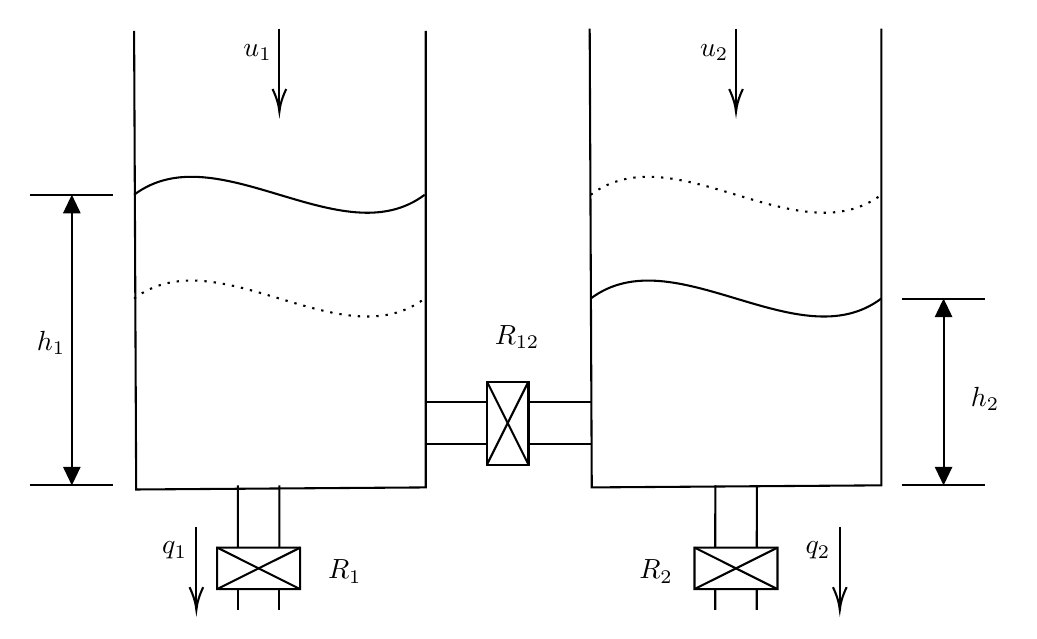
\begin{tikzpicture}[x=0.75pt,y=0.75pt,yscale=-1,xscale=1]
    %uncomment if require: \path (0,459); %set diagram left start at 0, and has height of 459
    %Straight Lines [id:da5688929335924803]
    \draw    (310.5,121) -- (310.5,341) -- (171,342) -- (170,121) ;
    %Straight Lines [id:da5444294116492245]
    \draw    (530,120) -- (530,340) -- (390.5,341) -- (389.5,120) ;
    %Straight Lines [id:da5805131124126722]
    \draw    (200,360) -- (200,398) ;
    \draw [shift={(200,400)}, rotate = 270] [color={rgb, 255:red, 0; green, 0; blue, 0 }  ][line width=0.75]    (10.93,-3.29) .. controls (6.95,-1.4) and (3.31,-0.3) .. (0,0) .. controls (3.31,0.3) and (6.95,1.4) .. (10.93,3.29)   ;
    %Straight Lines [id:da36945578968673487]
    \draw    (510,360) -- (510,398) ;
    \draw [shift={(510,400)}, rotate = 270] [color={rgb, 255:red, 0; green, 0; blue, 0 }  ][line width=0.75]    (10.93,-3.29) .. controls (6.95,-1.4) and (3.31,-0.3) .. (0,0) .. controls (3.31,0.3) and (6.95,1.4) .. (10.93,3.29)   ;
    %Straight Lines [id:da3077937138084411]
    \draw    (310,300) -- (340,300) ;
    %Straight Lines [id:da6773172185122848]
    \draw    (310,320) -- (340,320) ;
    %Shape: Rectangle [id:dp35476624369345366]
    \draw   (340,290) -- (360,290) -- (360,330) -- (340,330) -- cycle ;
    %Straight Lines [id:da9030142425581202]
    \draw    (360,300) -- (390,300) ;
    %Straight Lines [id:da9329287059080266]
    \draw    (360,320) -- (390,320) ;
    %Straight Lines [id:da7833363422326105]
    \draw    (340,290) -- (360,330) ;
    %Straight Lines [id:da26540765973372593]
    \draw    (360,290) -- (340,330) ;
    %Straight Lines [id:da7238601427391023]
    \draw    (470.02,340) -- (470,370) ;
    %Straight Lines [id:da21192498383993508]
    \draw    (450.02,339.99) -- (450,369.99) ;
    %Shape: Rectangle [id:dp4746471043409347]
    \draw   (480,370.01) -- (479.99,390.01) -- (439.99,389.98) -- (440,369.98) -- cycle ;
    %Straight Lines [id:da6336671048955647]
    \draw    (470,389.99) -- (469.98,400) ;
    %Straight Lines [id:da6700066277567417]
    \draw    (450,389.99) -- (449.98,400) ;
    %Straight Lines [id:da928718960478936]
    \draw    (480,370.01) -- (439.99,389.98) ;
    %Straight Lines [id:da1540497075962557]
    \draw    (479.99,390.01) -- (440,369.98) ;
    %Straight Lines [id:da7575667165517417]
    \draw    (240.03,340.01) -- (240.01,370.01) ;
    %Straight Lines [id:da24987185404211631]
    \draw    (220.03,340) -- (220.01,370) ;
    %Shape: Rectangle [id:dp2771887371908066]
    \draw   (250.01,370.02) -- (250,390.02) -- (210,389.99) -- (210.01,369.99) -- cycle ;
    %Straight Lines [id:da9912034440398235]
    \draw    (240,390) -- (240,400) ;
    %Straight Lines [id:da11904000202181764]
    \draw    (220,390) -- (220,400) ;
    %Straight Lines [id:da7480508238760858]
    \draw    (250.01,370.02) -- (210,389.99) ;
    %Straight Lines [id:da7049908339863217]
    \draw    (250,390.02) -- (210.01,369.99) ;
    %Straight Lines [id:da9101133488343268]
    \draw    (240,120) -- (240,158) ;
    \draw [shift={(240,160)}, rotate = 270] [color={rgb, 255:red, 0; green, 0; blue, 0 }  ][line width=0.75]    (10.93,-3.29) .. controls (6.95,-1.4) and (3.31,-0.3) .. (0,0) .. controls (3.31,0.3) and (6.95,1.4) .. (10.93,3.29)   ;
    %Straight Lines [id:da11474588029910615]
    \draw    (460,120) -- (460,158) ;
    \draw [shift={(460,160)}, rotate = 270] [color={rgb, 255:red, 0; green, 0; blue, 0 }  ][line width=0.75]    (10.93,-3.29) .. controls (6.95,-1.4) and (3.31,-0.3) .. (0,0) .. controls (3.31,0.3) and (6.95,1.4) .. (10.93,3.29)   ;
    %Curve Lines [id:da10596831311641142]
    \draw    (170,200) .. controls (210,170) and (270,230) .. (310,200) ;
    %Curve Lines [id:da32042097611565956]
    \draw    (390,250) .. controls (430,220) and (490,280) .. (530,250) ;
    %Curve Lines [id:da9628648357071894]
    \draw  [dash pattern={on 0.84pt off 2.51pt}]  (170,250) .. controls (210,220) and (270,280) .. (310,250) ;
    %Curve Lines [id:da13605436176729158]
    \draw  [dash pattern={on 0.84pt off 2.51pt}]  (390,200) .. controls (430,170) and (490,230) .. (530,200) ;
    %Straight Lines [id:da6375240487876032]
    \draw    (140,202) -- (140,338) ;
    \draw [shift={(140,340)}, rotate = 270] [fill={rgb, 255:red, 0; green, 0; blue, 0 }  ][line width=0.75]  [draw opacity=0] (8.93,-4.29) -- (0,0) -- (8.93,4.29) -- cycle    ;
    \draw [shift={(140,200)}, rotate = 90] [fill={rgb, 255:red, 0; green, 0; blue, 0 }  ][line width=0.75]  [draw opacity=0] (8.93,-4.29) -- (0,0) -- (8.93,4.29) -- cycle    ;
    %Straight Lines [id:da08454244898673535]
    \draw    (120,200) -- (160,200) ;
    %Straight Lines [id:da6622529040678575]
    \draw    (120,340) -- (160,340) ;
    %Straight Lines [id:da8094387172838741]
    \draw    (560,252) -- (560,338) ;
    \draw [shift={(560,340)}, rotate = 270] [fill={rgb, 255:red, 0; green, 0; blue, 0 }  ][line width=0.75]  [draw opacity=0] (8.93,-4.29) -- (0,0) -- (8.93,4.29) -- cycle    ;
    \draw [shift={(560,250)}, rotate = 90] [fill={rgb, 255:red, 0; green, 0; blue, 0 }  ][line width=0.75]  [draw opacity=0] (8.93,-4.29) -- (0,0) -- (8.93,4.29) -- cycle    ;
    %Straight Lines [id:da5524739963534533]
    \draw    (540,250) -- (580,250) ;
    %Straight Lines [id:da7800336719151444]
    \draw    (540,340) -- (580,340) ;
    % Text Node
    \draw (189.5,371.5) node  [align=left] {$\displaystyle q_{1}$};
    % Text Node
    \draw (499.5,371.5) node  [align=left] {$\displaystyle q_{2}$};
    % Text Node
    \draw (354.5,268.5) node  [align=left] {$\displaystyle R_{12}$};
    % Text Node
    \draw (229.5,131.5) node  [align=left] {$\displaystyle u_{1}$};
    % Text Node
    \draw (449.5,131.5) node  [align=left] {$\displaystyle u_{2}$};
    % Text Node
    \draw (130,271.5) node  [align=left] {$\displaystyle h_{1}$};
    % Text Node
    \draw (580,298.5) node  [align=left] {$\displaystyle h_{2}$};
    % Text Node
    \draw (271.5,381.5) node  [align=left] {$\displaystyle R_{1}$};
    % Text Node
    \draw (421.5,381.5) node  [align=left] {$\displaystyle R_{2}$};
  \end{tikzpicture}%
  }
  \caption[System of Coupled Tanks.]{System of Coupled Tanks. Two pumps input
    water into the system, and the water can flow out of the system through each
    tank. The water can also flow from one tank to another, making the state of
    one affect the state of the other. The control objective are the water
    levels of both tanks. The solid and dashed lines representing the water
    levels illustate two configurations, one with \(h_{1}>h_{2}\) and the
    contrary.}%
  \label{fig:tanks-sim}
\end{figure}


The output flow of the \(T1\) and \(T2\) are denoted by \(q_1\) and \(q_2\)
(\si{\cubic\centi\metre\per\second}), respectively, and the flow between them is
noted by \(q_{12}\) (\si{\cubic\centi\metre\per\second}). Both tanks have the
same cross-section area, denoted as \(A\) (\si{\square\centi\metre}), as well as the
cross-section areas of the restrictions in the outputs of the tanks, \(a\)
(\si{\square\centi\metre}); \(g\) (\si{\centi\metre\per\square\second}) is the gravity
acceleration. By using Bernoulli's equations, we have:
%
\begin{equation}
  \label{eq:formula-height-variation-lin}
  \begin{aligned}
    \dot{h}_1(t) & = \frac{u_1(t)-q_1(t)\pm{}q_{12}}{A}, \\
    \dot{h}_2(t) & = \frac{u_2(t)-q_2(t)\mp{}q_{12}}{A},
  \end{aligned}
\end{equation}
%
where the flows are given by \(q_1(t) = a\sqrt{2gh_1(t)}\),
\(q_2(t) = a\sqrt{2gh_2(t)}\), and
\(q_{12}(t) = a\sqrt{2g\left|h_2(t)-h_1(t)\right|}\).

This is a nonlinear and switching system, as the model changes depending on the
height of the tanks' water column. At each mode, \(h_1>h_2\) or \(h_1\leq h_2\),
equation~\eqref{eq:formula-height-variation-lin} can be linearized around an
equilibrium operational point \((x_{eq},u_{eq})\) by using Jacobian matrices. In
what follows, we use \(a=\SI{5.9}{\centi\metre\squared}\),
\(A=\SI{961\pi{}}{\centi\metre\squared}\), and
\(g=\SI{980.665}{\centi\metre\per\square\second}\).

Two operational conditions with
\(x(k) = \begin{bmatrix}h_1(k) & h_2(k)\end{bmatrix}^\top{}\), chosen so one tank
is nearly full, are such that:
%
\begin{equation*}
  x_{eq}^1 =\! \begin{bmatrix}
    57.5 \\ 43.61
  \end{bmatrix}\!,
  u_{eq}^1 =\! \begin{bmatrix}
    744 \\ 2960
  \end{bmatrix}\!,
  x_{eq}^2 = \begin{bmatrix}
    43.61 \\ 57.5
  \end{bmatrix}\!,
  u_{eq}^2 =\! \begin{bmatrix}
    2960 \\ 744
  \end{bmatrix}\!,
\end{equation*}
%
yielding two operational modes, each of them corresponding to a \CG{}.\@
%
After the linearization, we discretized the continuous-time model using a sample
time of \SI{5}{\second} and Euler equations to get discrete-time model given
by~\eqref{eq:state-space} with matrices:
%
\begin{align*}
  A_1 & =
  \begin{bmatrix}
    0.92  & 0.053 \\
    0.053 & 0.91
  \end{bmatrix}, ~~~ A_2 = \begin{bmatrix}
    0.91  & 0.053 \\
    0.053 & 0.92
  \end{bmatrix} \\
  B_1 & =
  \begin{bmatrix}
    0.0016           & 4.5\times10^{-5} \\
    4.5\times10^{-5} & 0.0016
  \end{bmatrix},
  B_2 = \begin{bmatrix}
    0.0016           & 4.5\times10^{-5} \\
    4.5\times10^{-5} & 0.0016
  \end{bmatrix},                              \\
  %
  C_1 & = C_2 =
  \begin{bmatrix}
    1 & 0 \\
    0 & 1
  \end{bmatrix},
\end{align*}
%
and number of modes \(s=2\). Using Lyapunov's
approach~\parencite{chen:linear,hespanha:linear}, on the system augmented with 2
integrators (one for each state), we got the following controller:
%
\begin{align*}
  K_1 & = \begin{bmatrix}
    -875.384 & -9.217   & -297.447 & 7.982    \\
    -8.505   & -849.853 & 8.514    & -279.434
  \end{bmatrix}, \\
  %
  K_2 & = \begin{bmatrix}
    -849.853 & -8.505   & -279.434 & 8.514    \\
    -9.217   & -875.384 & 7.982    & -297.447
  \end{bmatrix},
\end{align*}
%
for the operational modes \(1\) and \(2\).

We simulated our approaches described by Algorithm~\ref{alg:roa-rule} to switch
between the \CG{}s 1 and 2. In both cases the system starts in \(x(0) =
\begin{bsmallmatrix}43.61 & 57.5\end{bsmallmatrix}^{\top}\). The references are
\(r = \begin{bsmallmatrix}57.5 & 43.61\end{bsmallmatrix}^{\top}\), for
\(0\leq k\leq 10 \cup 50 \leq k \leq\infty{}\), and
\(r = \begin{bsmallmatrix}43.61& 57.5\end{bsmallmatrix}^{\top}\), for
\(11 \leq k \leq 49\). Therefore, the system must perform a closed path. Note that the
references are the system's two equilibrium points, so the systems starts in
mode 1, moves to mode 2 and goes back to mode 1.

The regions of attraction were estimated using the optimization procedure
presented in Section~\ref{sec:region-of-attraction}. The following inequalities
define each mode's regions of attraction:
%
\begin{align}
  \mathcal{L}_{V_{1}}(x) & = x^{\top} \begin{bmatrix}
    4.766\times{}10^{-3} & 1.431\times{}10^{-8} \\
    1.431\times{}10^{-8} & 4.766\times{}10^{-3}
  \end{bmatrix}x \leq 1 \\
  \mathcal{L}_{V_{2}}(x) & = x^{\top} \begin{bmatrix}
    4.766\times{}10^{-3} & 1.185\times{}10^{-8} \\
    1.185\times{}10^{-8} & 4.766\times{}10^{-3}
  \end{bmatrix}x \leq 1
\end{align}

The constraint regions are, in this case, also defined as ellipses, given by the
following inequalities:
%
\begin{align}
  \mathcal{C}_{1}(x) & = \frac{(x_{1}-50.55)^{2}}{8.681^{2}} + \frac{(x_{2}-43.61)^{2}}{1.085^{2}} \leq 1 \\
  \mathcal{C}_{2}(x) & = \frac{(x_{1}-43.61)^{2}}{1.085^{2}} + \frac{(x_{2}-50.55)^{2}}{8.681^{2}} \leq 1
\end{align}
%
where \(x=\begin{bsmallmatrix} x_{1} & x_{2} \end{bsmallmatrix}^{\top}\).

Since the system is linearized around two different operation points, there are
three bases (the equilibrium points of each linearized model), and the states
need to be converted between them. The first is the basis of the non-linear
system, called \enquote{global}. The second and third are those of the
linearized systems. The constraints are written on the global basis and the
regions of attraction in the respective mode's basis. Care must be taken to
convert between the basis for set membership tests.

Fig.~\ref{fig:states} shows the path taken by the closed-loop system over the
space of the system's state. The trajectory marked with
\textcolor{red}{red-dashed line} concerns the results achieved without
early-switch, and the \textcolor{blue}{solid-blue line} is related to ones with
early-switch. The shadow regions concern the constraints of each mode. Also,
Fig.~\ref{fig:states} shows the borders of the estimates of the regions of
attraction, RoA, for each mode, with dot-dashed lines.

It is clear that the path taken under each algorithm's variation (with and
without early controller switch) are almost the same. The respective control
signals are given in Fig.~\ref{fig:control-signals}, showing faster convergence
and smaller signal amplitude in the hybrid switch.

\begin{figure}[ht!]
  \centering
  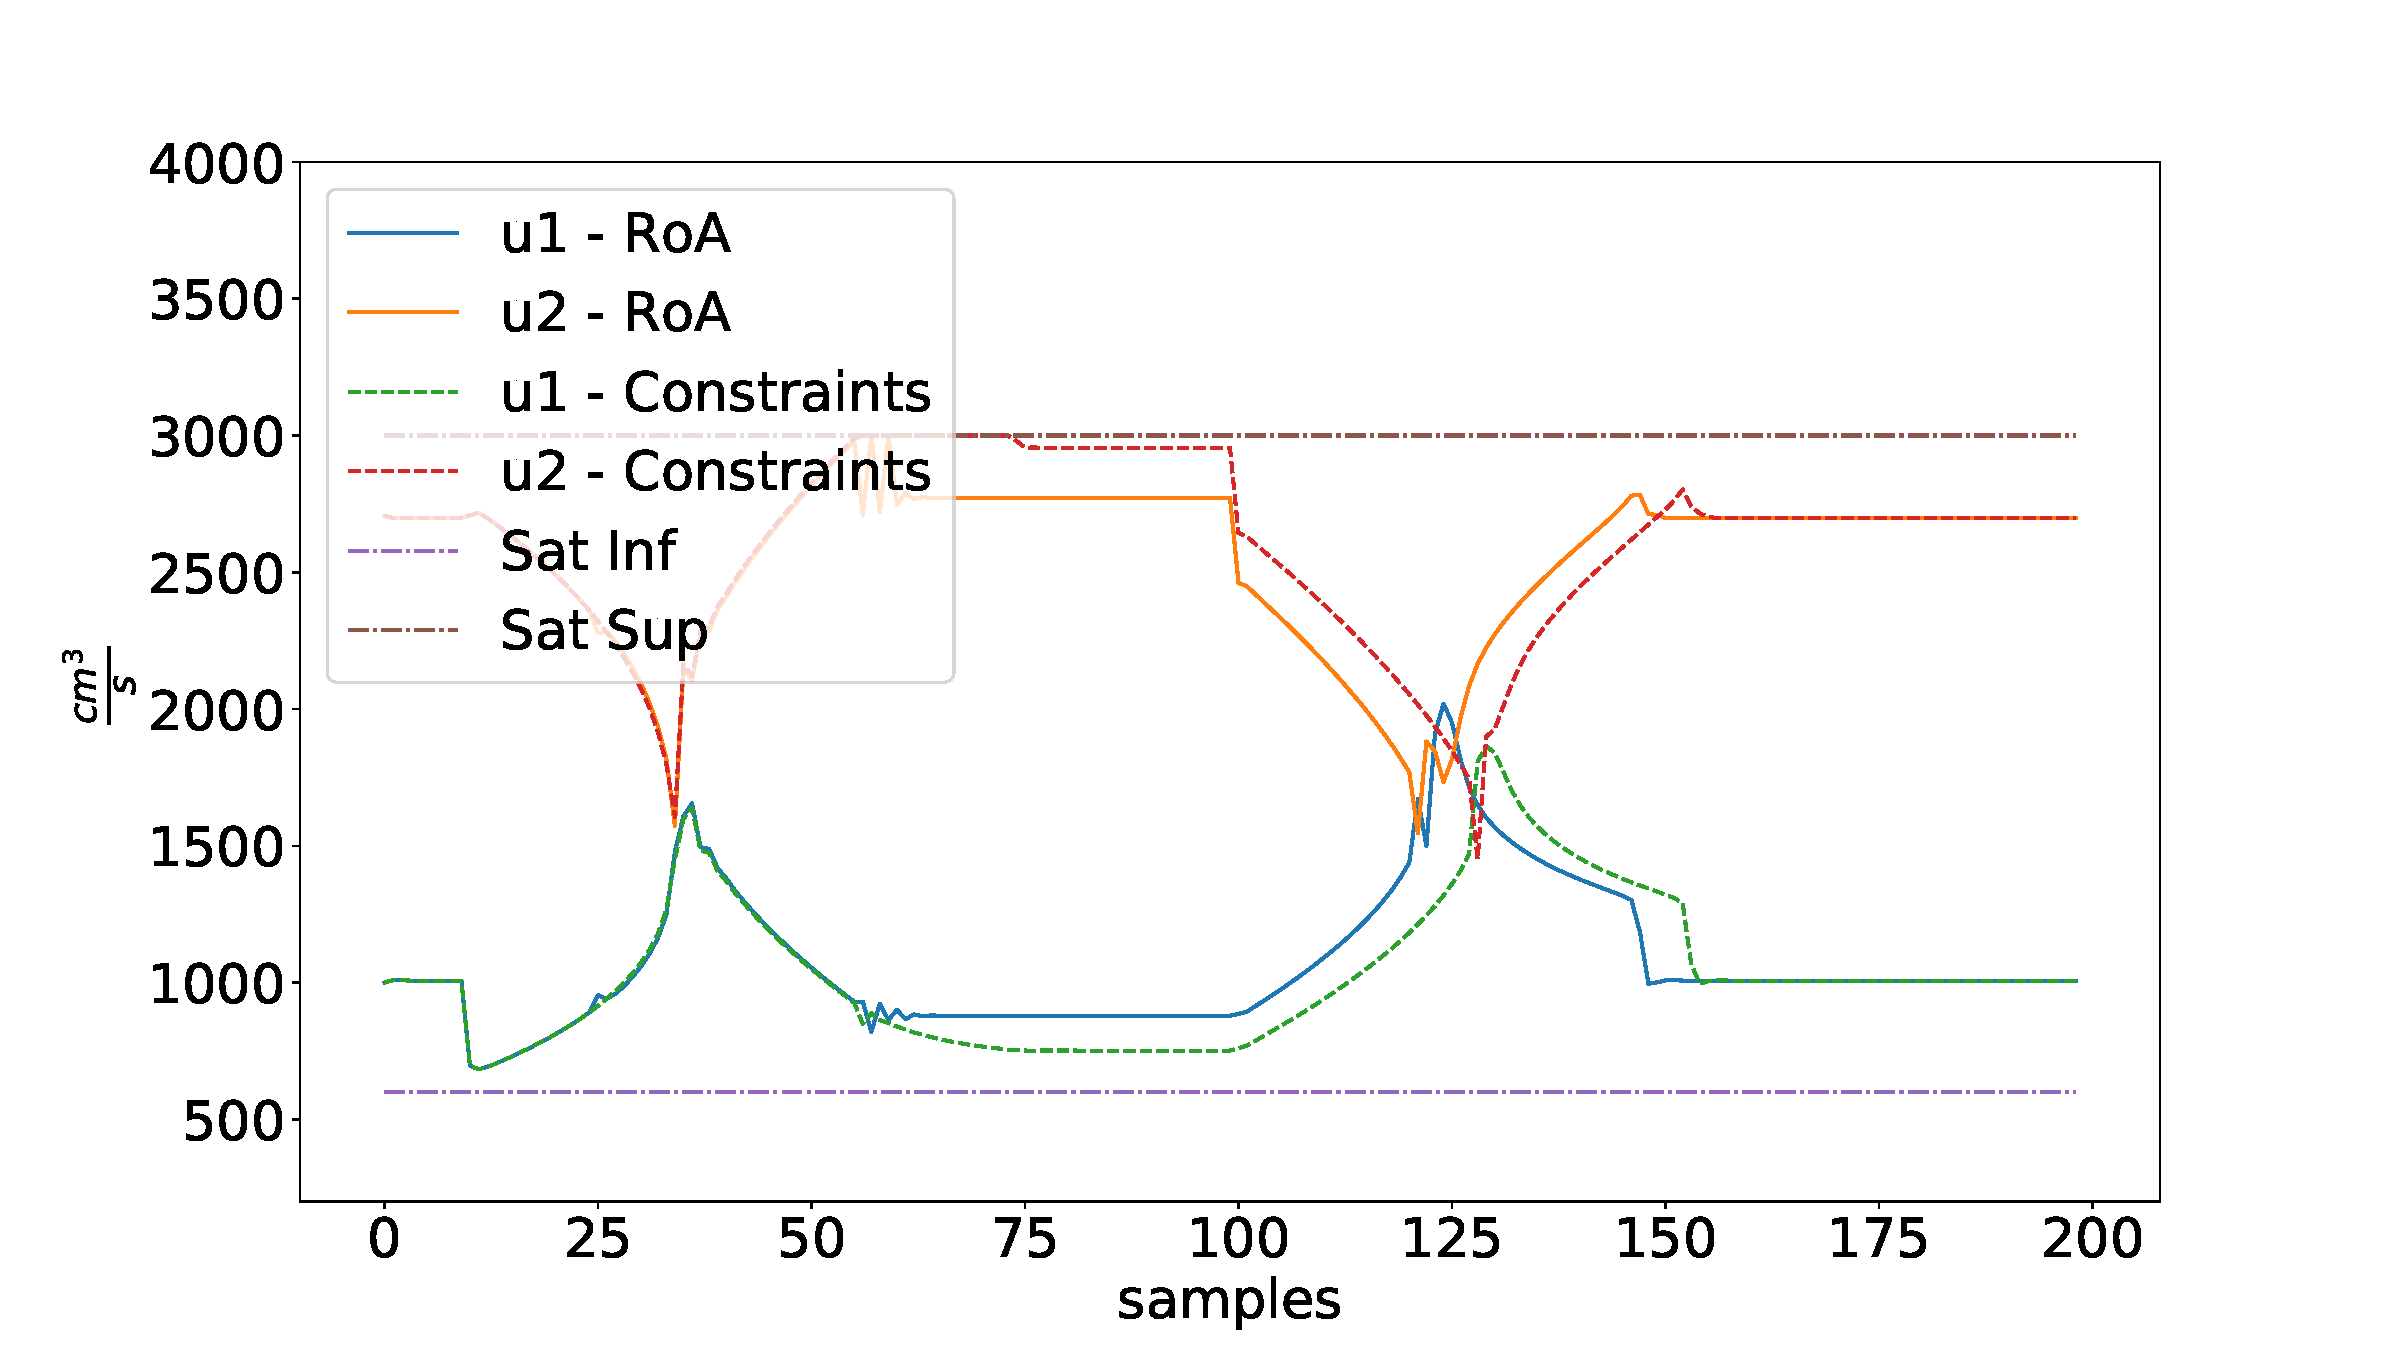
\includegraphics[width=0.8\linewidth]{imgs/tanks-control-signal}
  \caption[Control signals for Example 1.]{Control signals for Example 1. Solid
    lines are the hybrid switch and dashed lines are the normal switch.
    Dashed-dotted lines are saturations.}%
  \label{fig:control-signals}
\end{figure}

\begin{figure}[ht!]
  \centering
  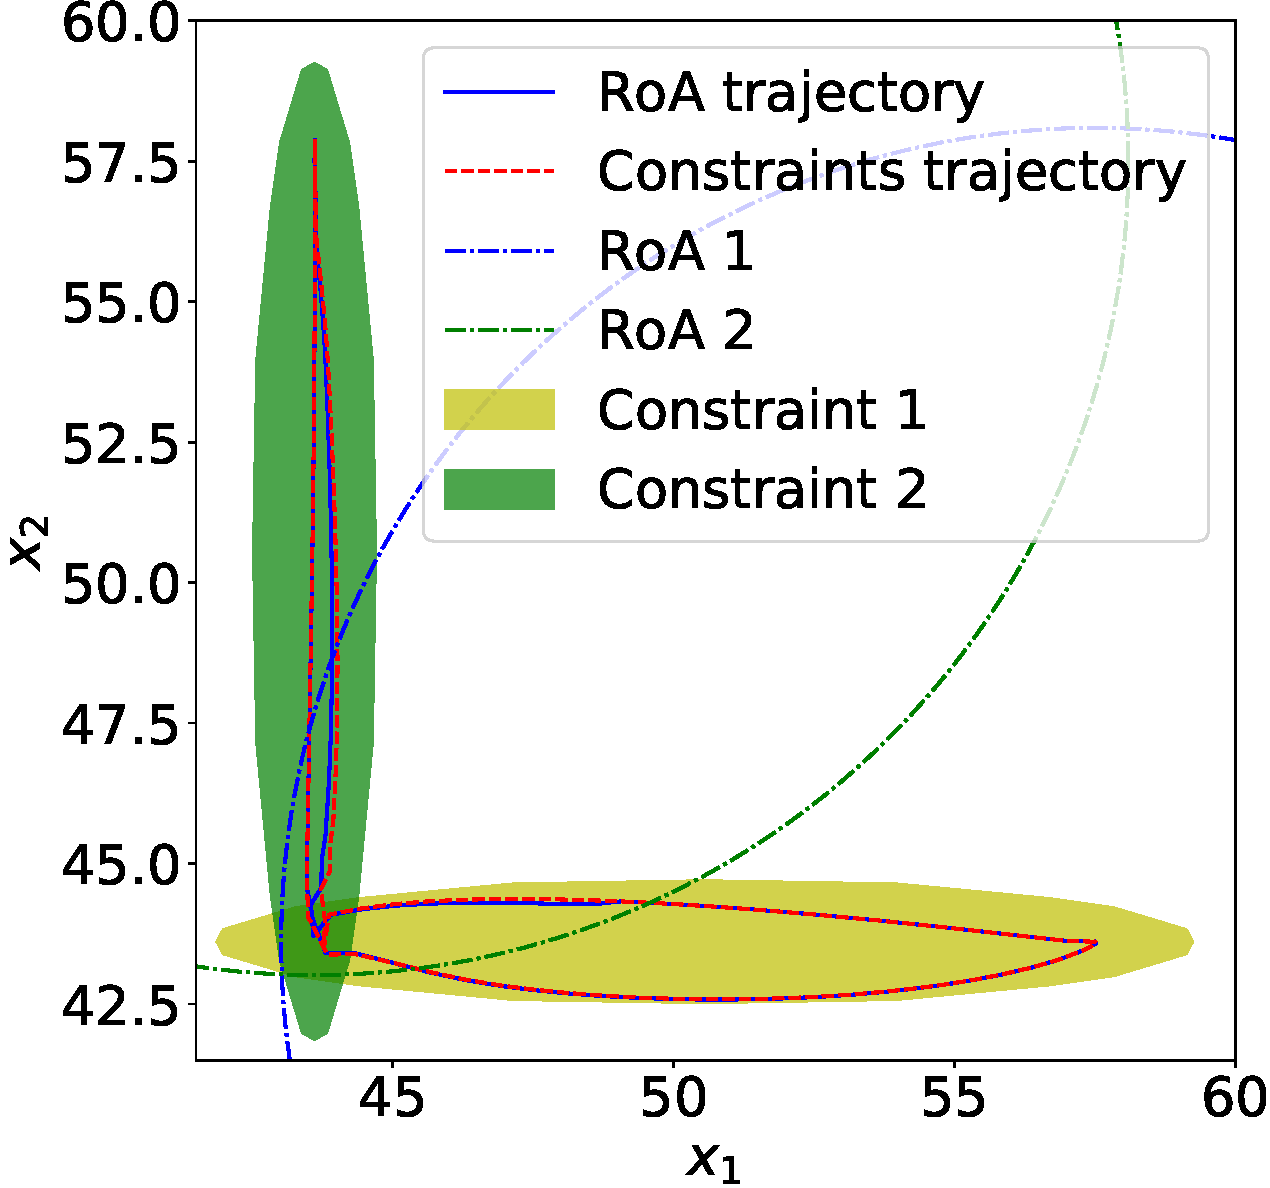
\includegraphics[width=0.9\linewidth]{imgs/tanks-states}
  \caption[States trajectory for Example 1.]{States trajectory for Example 1.
    The filled ellipses are each mode's constraints. The dashed-dotted circles
    are each controller's Region of Attraction. The dashed blue red line is the
    state path of the normal switch and the solid blue line the state path of
    the hybrid switch.}%
  \label{fig:states}
\end{figure}

\FloatBarrier

\subsection{Unstable System}%
\label{subsec:unstable-system}

Consider the unstable switching system with matrices
%
\begin{align*}
  A_1 & =
  \begin{bmatrix}
    1 & 0.003 \\
    0 & 1
  \end{bmatrix},
  A_2 = \begin{bmatrix}
    1 & 0.0074 \\
    0 & 1.1
  \end{bmatrix}, \\
  B_1 & =
  \begin{bmatrix}
    0.0005 & 1.2\times{}10^{-6} \\
    0      & 0.0008
  \end{bmatrix},
  B_2 = \begin{bmatrix}
    0.0019 & 3.6\times{}10^{-5} \\
    0      & 0.011
  \end{bmatrix}, \\
  %
  C_1 & = C_2 =
  \begin{bmatrix}
    1 & 0 \\
    0 & 1
  \end{bmatrix},       \\
\end{align*}
%
and operational points
%
\[
  x_{eq}^1 = \begin{bmatrix}
    1 \\ 1
  \end{bmatrix},
  u_{eq}^1 = \begin{bmatrix}
    -2 \\ \frac{-5}{4}
  \end{bmatrix},
  x_{eq}^2 = \begin{bmatrix}
    -1 \\ 1
  \end{bmatrix},
  u_{eq}^2 = \begin{bmatrix}
    \frac{-30}{19} \\ -10
  \end{bmatrix}.
\]
%
The sample-period was \SI{0.1}{\second}, and controller gains are given by:
%
\scriptsize
\begin{align*}
  K_1 & = \begin{bmatrix}
    -2.669\times{}10^3   & -1.993             & -6.741\times{}10^2    & 1.010              \\
    3.582\times{}10^{-4} & -1.669\times{}10^3 & -3.103\times{}10^{-4} & -4.210\times{}10^2
  \end{bmatrix}, \\
  %
  K_2 & = \begin{bmatrix}
    -7.034\times{}10^2    & -1.268             & -1.769\times{}10^2    & 6.097\times{}10^{-1} \\
    -3.903\times{}10^{-6} & -1.370\times{}10^2 & -1.292\times{}10^{-5} & -3.202\times{}10^1
  \end{bmatrix}.
\end{align*}
\normalsize

With the same procedures and considerations of the previous example, including
the used color codes, we simulated the unstable system.
Figure~\ref{fig:unstable-states} shows the same system trajectory for both
methods.

\begin{figure}[ht!]
  \centering
  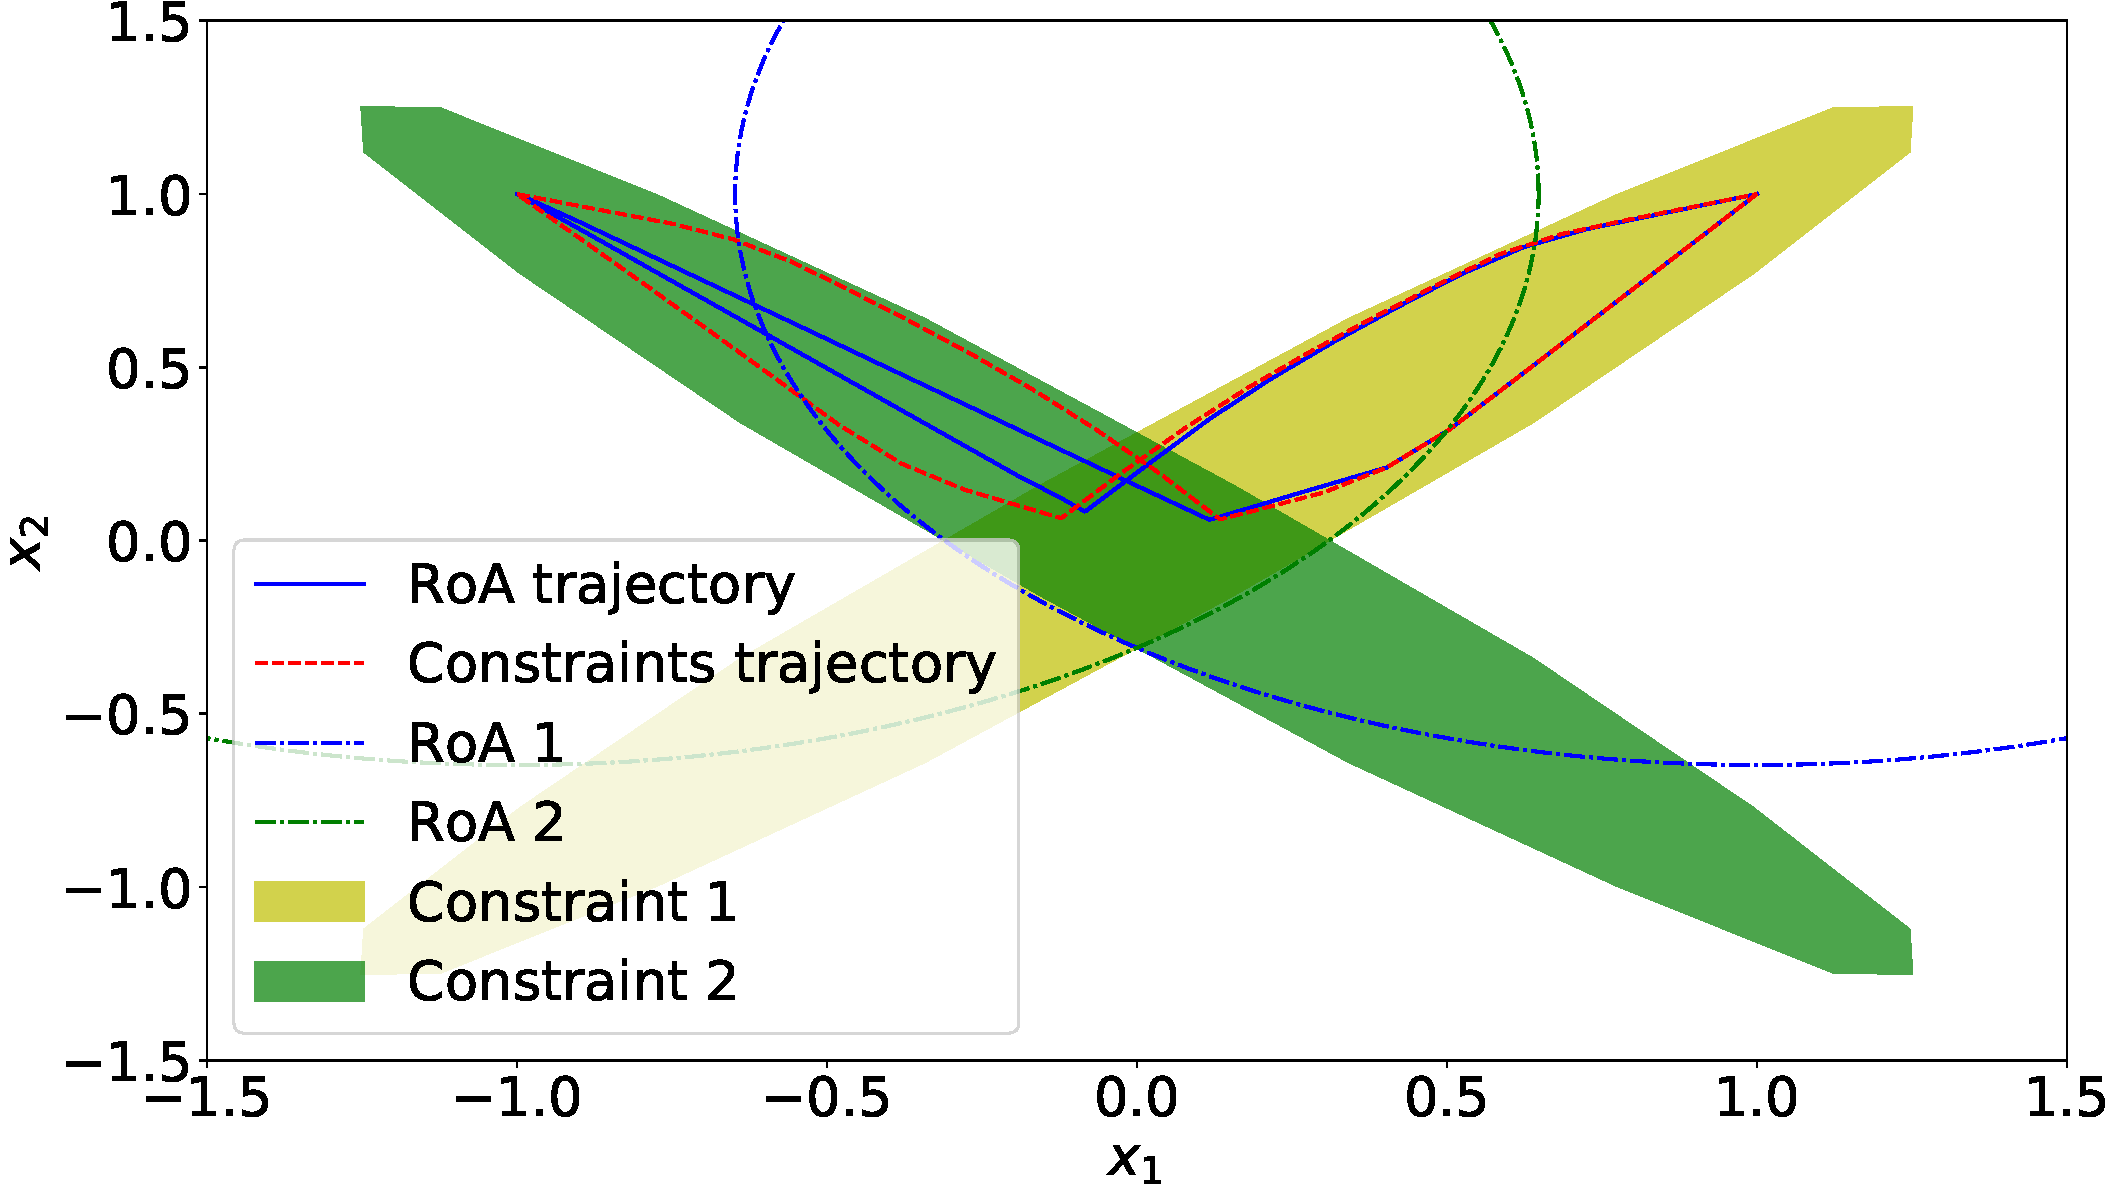
\includegraphics[width=\linewidth]{imgs/unstable_states}
  \caption[States trajectory for Example 2.]{States trajectory for Example 2.
    The filled ellipses are each mode's constraints. The dashed-dotted circles
    are each controller's Region of Attraction. The dashed blue red line is the
    state path of the normal switch and the solid blue line the state path of
    the hybrid switch.}%
  \label{fig:unstable-states}
\end{figure}

The second method shows better performance under control signal restrictions.
Figure~\ref{fig:unstable-control-signals} reveals a difference in the control
signals, where the first method, displayed in \textcolor{red}{red dashed-line}
and \textcolor{green}{green dashed-line}, have higher control signal outputs
than the second method, shown by \textcolor{blue}{blue solid-line} and
\textcolor{orange}{orange solid-line}. Both methods results in the same settling
time, but with much lower control effort with the strategy of early switching.

\begin{figure}[ht!]
  \centering
  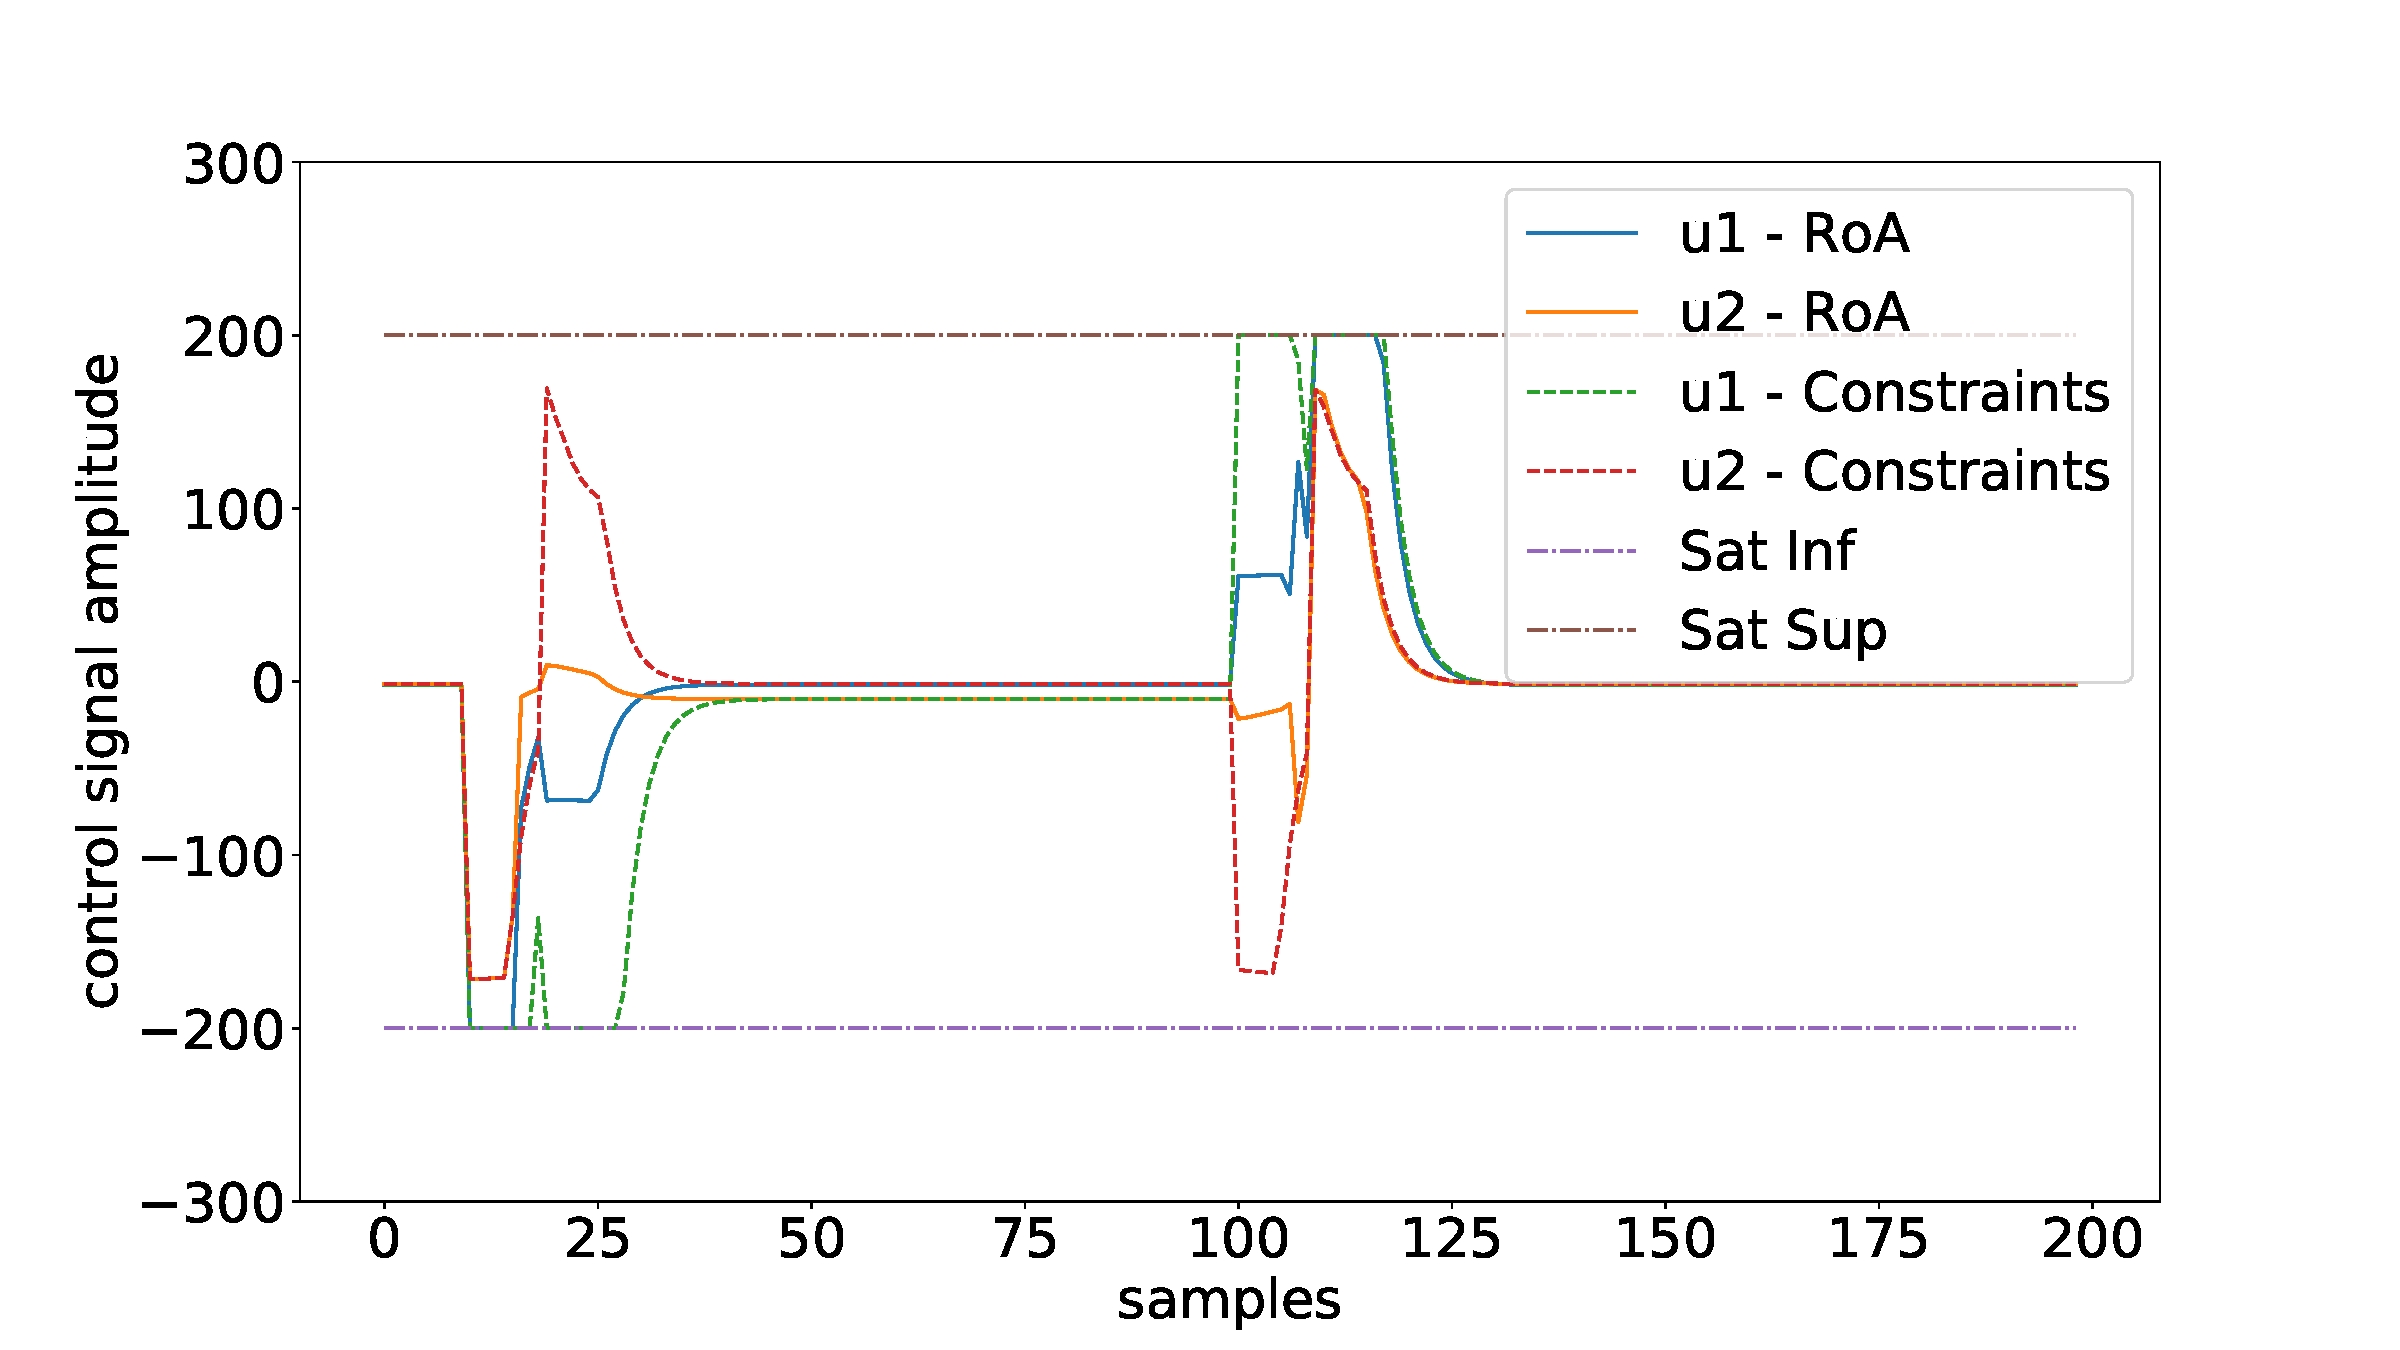
\includegraphics[width=\linewidth]{imgs/unstable_control_signal}
  \caption[Control signals for Example 2.]{Control signals for Example 2. Solid
    lines are the hybrid switch and dashed lines are the normal switch.
    Dashed-dotted lines are saturations.}%
  \label{fig:unstable-control-signals}
\end{figure}

\FloatBarrier

\subsection{Cessna 182}%
\label{subsec:cessna}

\textcite{franzè.lucia.ea:command} present a Cessna 182 aircraft model, which
they used to simulate a dwell-time. They describe the model, the operation
points they chose, and the constraints applied to it. We used the same system
changing only the switch technique to compare the performance. The proposed
technique took \SI{6}{\second} to converge, whereas the dwell-time technique
took over \SI{20}{\second}.

Figure~\ref{fig:cessna-u} shows both actuators' control signals, which are kept
mostly invariant, except at the mode transitions, where the integrator reset
created a discontinuity. Figure~\ref{fig:cessna-x} shows each state. In both
figures, the solid black lines at the plot's top and bottom are the signal's
constraints. The last state (\(x_{4}\)) is the output, and its plot also shows
the reference and command governor's output.

\begin{figure}[ht!]
  \centering
  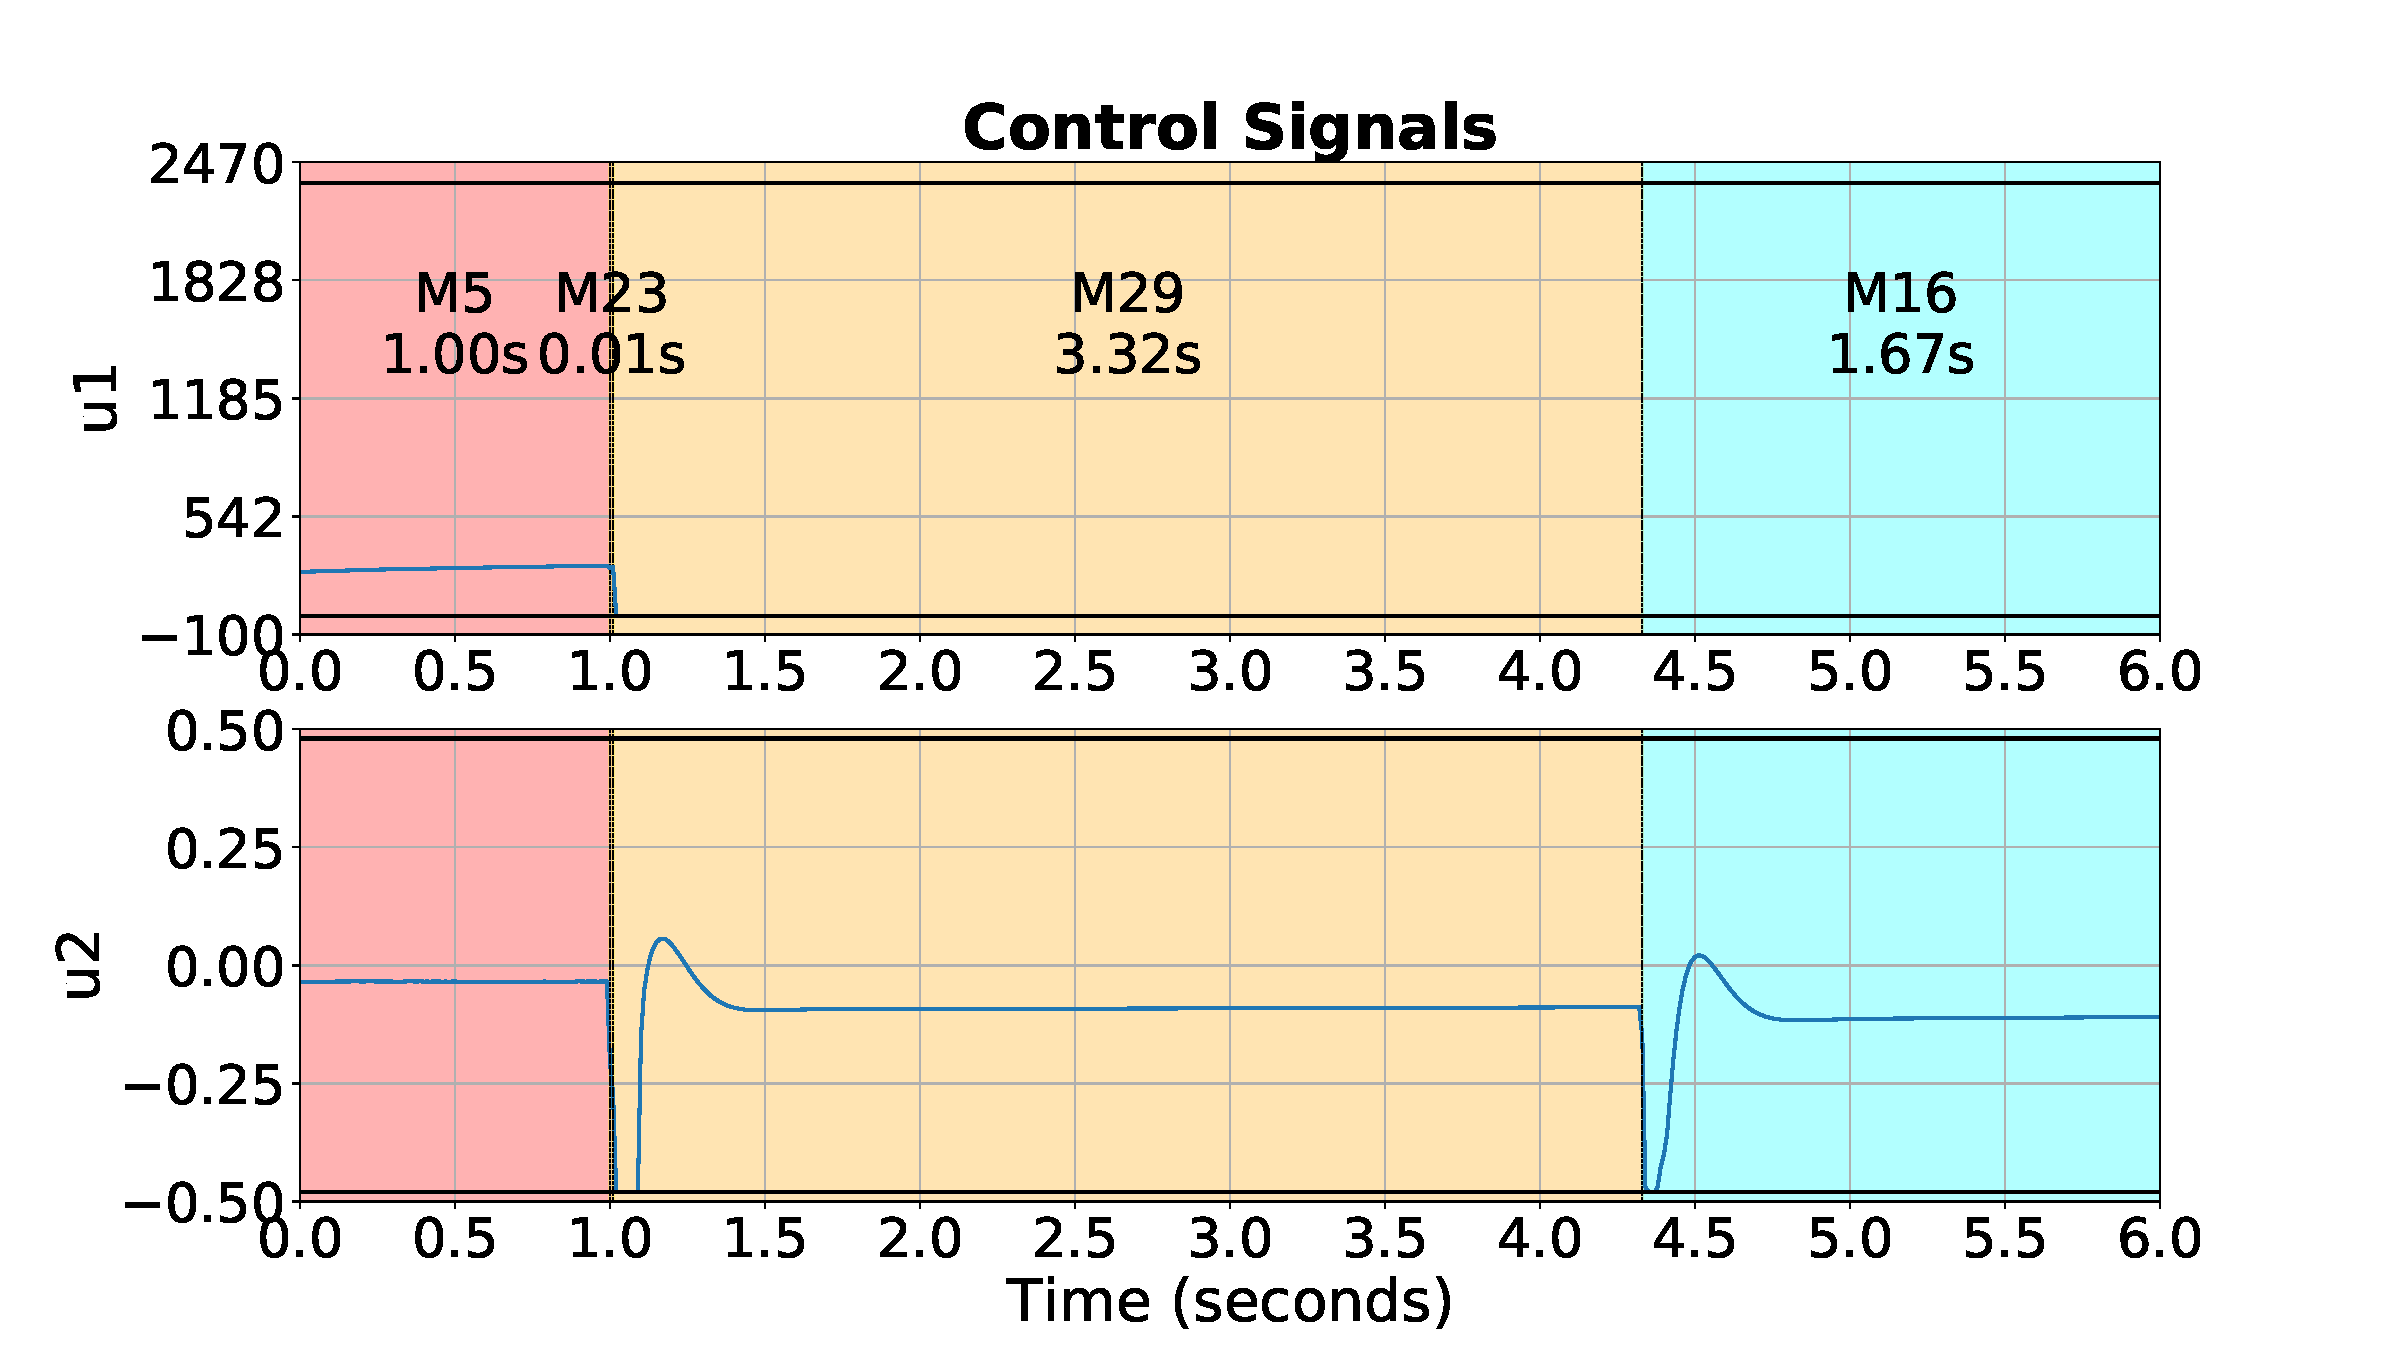
\includegraphics[height=0.3\textheight]{imgs/cessna-u}
  \caption{Cessna 192 control signals.}%
  \label{fig:cessna-u}
\end{figure}

\begin{figure}[ht!]
  \centering
  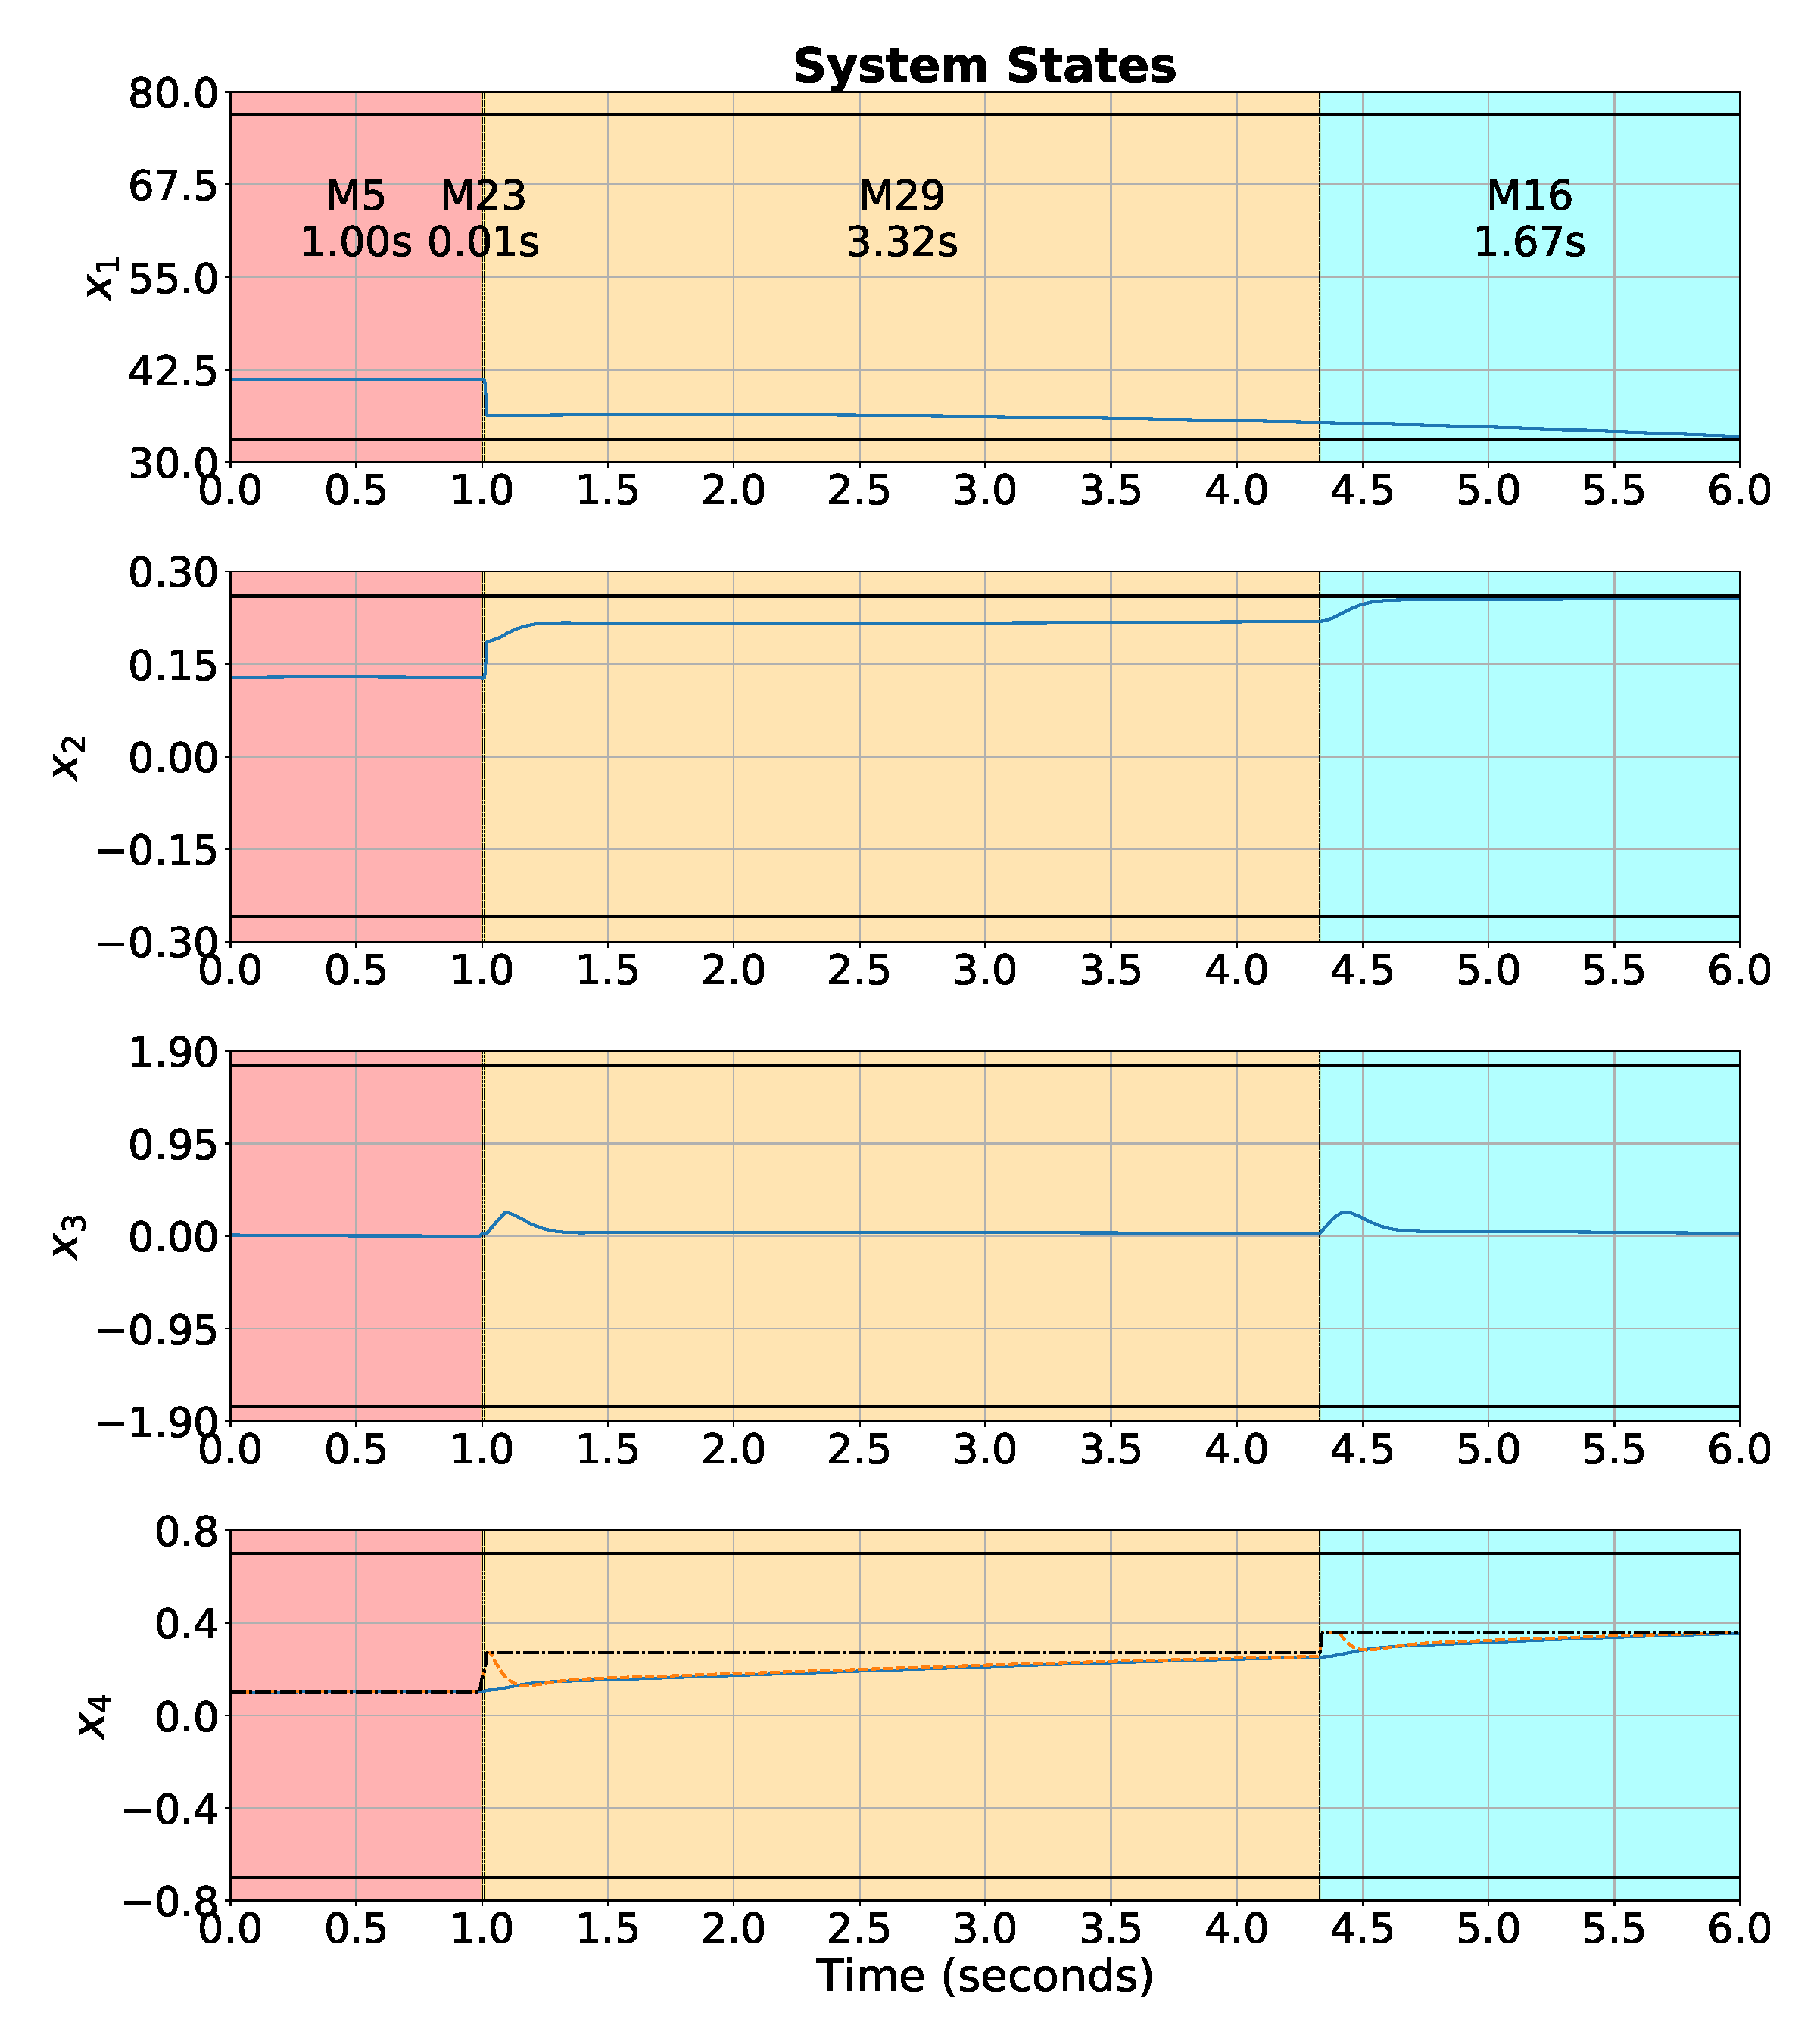
\includegraphics[height=0.6\textheight]{imgs/cessna-x}
  \caption[Cessna 182 states.]{Cessna 182 states. The colored backgrounds show
    the active mode. In the last plot, the dashed black line is the reference
    set by the supervisor, the dashed orange line is the reference generated by
    the Command Governor, the solid blue line is the state and the solid black
    lines are the saturation values.}%
  \label{fig:cessna-x}
\end{figure}

\section{Experimental Results}%
\label{sec:experimental-results}

Consider an interactive tank system as indicated in Figure~\ref{fig:tanks}. It
describes the physical system present at the System Analysis Laboratory of
CEFET-MG campus V, shown in Figure~\ref{fig:tanks-real}. It consists of two
coupled tanks, \(T1\) and \(T2\), that are fed by a pump with controlled flow
\(u(t)\), measured in \si{\cubic\centi\metre\per\second}. The levels of each
tank, \(h_1\) and \(h_2\) (\si{\centi\metre}), are the control objective
variables, and are measured
directly~\parencite{franco.oliveira.ea:síntese,sousa.leite.ea:affordable,lopes.leite.ea:anti-windup}.

\begin{figure}[ht!]
  \centering
  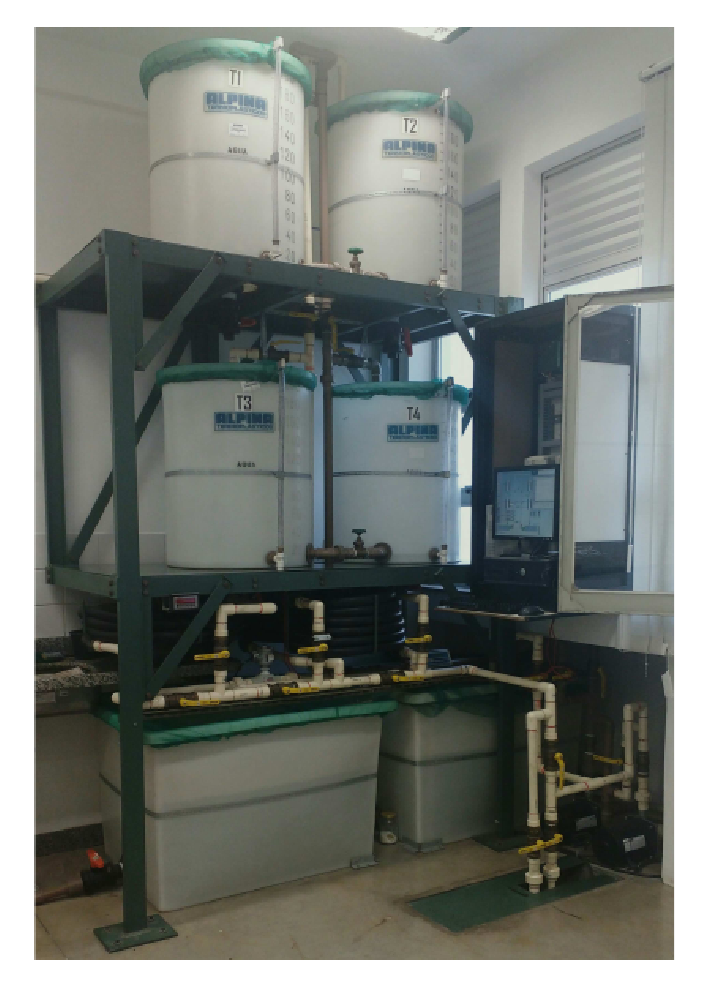
\includegraphics[height=.5\textheight]{imgs/tanks-real}
  \caption[System of coupled tanks.]{System of coupled tanks with four 200L
    tanks. There are two pumps that can be configured through the pipes to fill
    any of the tanks. Tank T3 has a rigid body with a non-linear shape inside
    it. The water flow between tanks is also configurable.}%
  \label{fig:tanks-real}
\end{figure}

\begin{figure}[ht!]
  \centering
  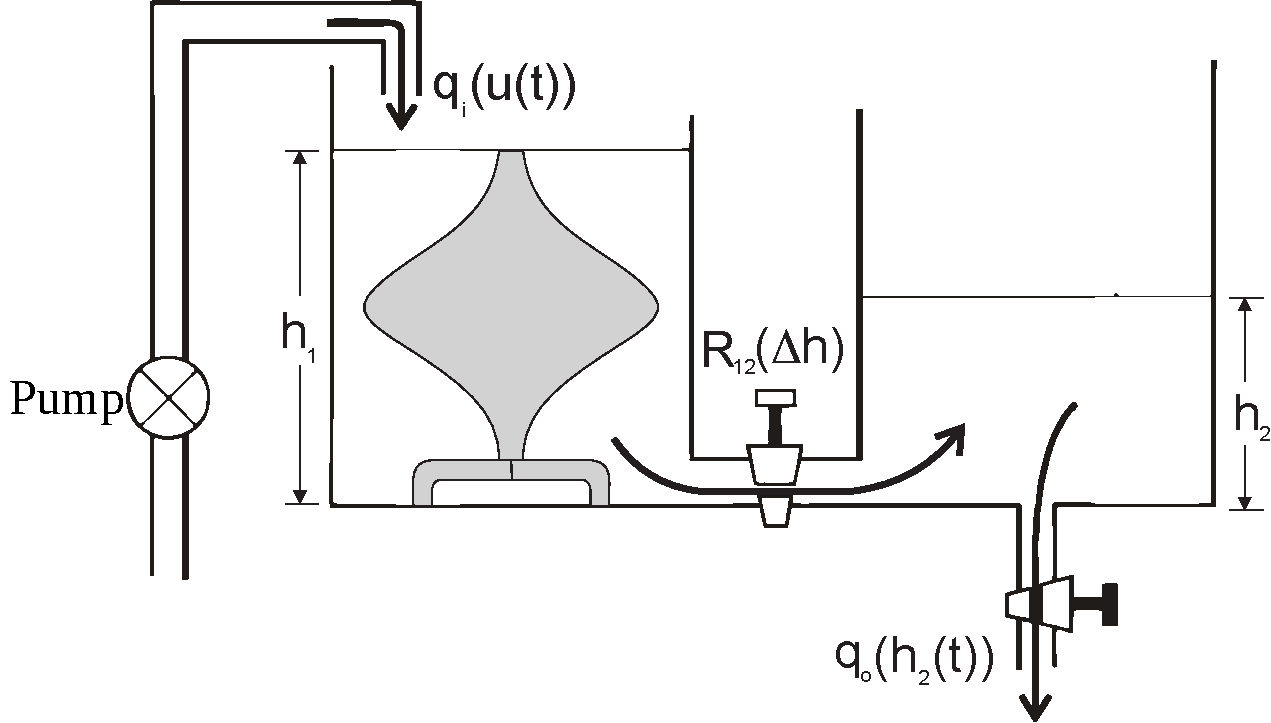
\includegraphics[width=0.9\linewidth]{imgs/tanks}
  \caption[Coupled tanks diagram.]{Diagram of the third and fourth tanks,
    showing the non-linear body. The water flows from the pump into the tank
    three, then move to tank four and goes back to the reservoir.}%
  \label{fig:tanks}
\end{figure}

Both tanks have the same cross-section area, denoted as \(A\)
(\si{\square\centi\metre}), however, there is a solid inside \(T1\) that makes its
area non-linear and adds uncertainties to its model. The cross-section area of
\(T1\) becomes
%
\begin{equation}
  \label{eq:t1-area}
  A_{1}(h_{1}(t)) = \frac{3r}{5} \left(
  2.7r - \frac{\cos(2.5\pi{}((h_{1}(t)-8)\times{}10^{-2}-\mu))}{\sigma{}\sqrt{2\pi}}
  e^{-\frac{((h_{1}(t)-8)\times{}10^{-2}-\mu^{2})^{2}}{2\sigma^{2}}}
  \right),
\end{equation}
%
where \(\mu=0.4\), \(\sigma=0.55\) and \(r=0.31\). The cross-section area of \(T2\) is
\(\SI{0.31}{\square\metre}\).

By using Bernoulli's equations, the system's dynamics can be described by:
%
\begin{equation}
  \label{eq:formula-height-variation}
  \begin{aligned}
    \dot{h}_1(t) & = \frac{R_{12}(h_{1}(t),h_{2}(t))\times{}K_{b}\times{}u(t)-h_{1}(t)+h_{2}(t)}
    {A_{1}(h_{1}(t))\times{}R_{12}(h_{1}(t),h_{2}(t))}                                                                 \\
    \dot{h}_2(t) & = \frac{h_{1}(t)-h_{2}(t)}{R_{12}(h_{1}(t),h_{2}(t))\times{}A_{2}} - \frac{q_{o}(h_{2}(t))}{A_{2}},
  \end{aligned}
\end{equation}
%
where \(R_{12}(h_{1}(t),h_{2}(t))=(0.412(h_{1}(t-h_{2}(t))+11.488)\times{}10^{-3}\)
and \(q_{o}(h_{2}(t))=11.941h_{2}(t)+787.586\). A frequency inverter controls
the pump through the percentage of maximum flow, and this value can be converted
to flow by \(q_{i}=13.201u_{t}+220.085\). Applying this before inputing in
Equation~\eqref{eq:formula-height-variation} results in \(u(t)\) becoming this
percentual value instead of the flow directly.

We chose four operation points to cover a significant portion of the available
\(h_{1}\) range (0 to \SI{70}{\centi\metre}), which is the output of the system.
The points and their respective linearized and discretized (with a sampling time
of \SI{5}{\second}) systems are

\begin{align*}
  \label{eq:op-points}
  \left[\begin{array}{c|c}
      x_{eq}^{\top} & u_{eq} \\
      \hline
      A             & B
    \end{array}\right]_{1} & = \left[\begin{array}{cc|c}
      19.5  & 5    & 15     \\
      \hline
      0.91  & 0.14 & 0.028  \\
      0.085 & 0.9  & 0.0013
    \end{array}\right],
  \left[\begin{array}{c|c}
      x_{eq}^{\top} & u_{eq} \\
      \hline
      A             & B
    \end{array}\right]_{2} & = \left[\begin{array}{cc|c}
      27.5  & 11.6 & 20     \\
      \hline
      0.94  & 0.19 & 0.04   \\
      0.084 & 0.9  & 0.0018
    \end{array}\right], \\
  \left[\begin{array}{c|c}
      x_{eq}^{\top} & u_{eq} \\
      \hline
      A             & B
    \end{array}\right]_{3} & = \left[\begin{array}{cc|c}
      37.3  & 17.8 & 25     \\
      \hline
      1.1   & 0.47 & 0.1    \\
      0.086 & 0.92 & 0.0042
    \end{array}\right],
  \left[\begin{array}{c|c}
      x_{eq}^{\top} & u_{eq} \\
      \hline
      A             & B
    \end{array}\right]_{4} & = \left[\begin{array}{cc|c}
      47.4  & 24.9 & 30     \\
      \hline
      0.49  & 0.96 & 0.22   \\
      0.053 & 0.95 & 0.0096
    \end{array}\right].
\end{align*}

To develop the controllers we applied the LMI described in the
Section~\ref{sec:region-of-attraction}~-~\nameref{sec:region-of-attraction} to
the integral-augmented system. The augmented state is the integral of the
output, \(h_{1}\). The points forced to be inside the region of attraction are
the previous' and next's operation point. It creates an intersection that allows
the early switching of controllers, which speeds up convergence. The following
controllers were obtained:

\begin{align}
  K_{1} & = \begin{bmatrix} -12.884 & -97.540 & -13.975 \end{bmatrix}, \\
  K_{2} & = \begin{bmatrix} -10.054 & -73.777 & -10.523 \end{bmatrix}, \\
  K_{3} & = \begin{bmatrix} -5.840  & -31.622 & -4.148 \end{bmatrix}, \\
  K_{4} & = \begin{bmatrix} -1.832  & -21.527 & -4.177 \end{bmatrix}.
\end{align}

To calculate each of the described modes' dwell-time, we applied the technique
described by~\textcite{franzè.lucia.ea:command}. We then ran both approaches ---
the dwell-time and the proposed one --- on the physical system.
Figures~\ref{fig:tanks-dwell} and~\ref{fig:tanks-roa} show the result of the
experiments, where the colored backgrounds represent the different modes, M1 to
M4, the two states (\(x_{1}\) and \(x_{2}\)) are plotted alongside their
respective real (\(r_{1,2}\)) and virtual (\(g_{1,2}\)) references.

The proposed technique has a faster overall convergence, entering the final mode
after 215 seconds while the dwell-time approach takes 340 seconds. This can
easily be seen by comparing the width of the regions with different background
colors, as the red, orange and yellow regions are much shorter on the proposed
technique. The proposed approach also shows no overshoot, since it does not give
the system enough time to converge to the waypoints and keeps it always moving
towards the reference, as shown by the states' trajectories, which are always
moving torwards the reference in the proposed technique, but starts to converge
to the mode's operation point on the dwell-time technique. Because of that, it
also has a smaller control effort, producing smaller control signal variation,
seen in the last plot, where the control signal constantly saturates in the
dwell-time approach, but does not saturate and has a smaller variation in the
proposed technique.

The last mode should also have an overshoot on the proposed technique, since it
is part of the closed-loop dynamics. However, the command governor's
optimization problem generated virtual references that slowly guided the system
to the real reference, making it take longer than necessary to converge. The
behaviour was present on every test repetition, just like the dwell-time
approach's overshoots.

\begin{figure}[ht!]
  \centering
  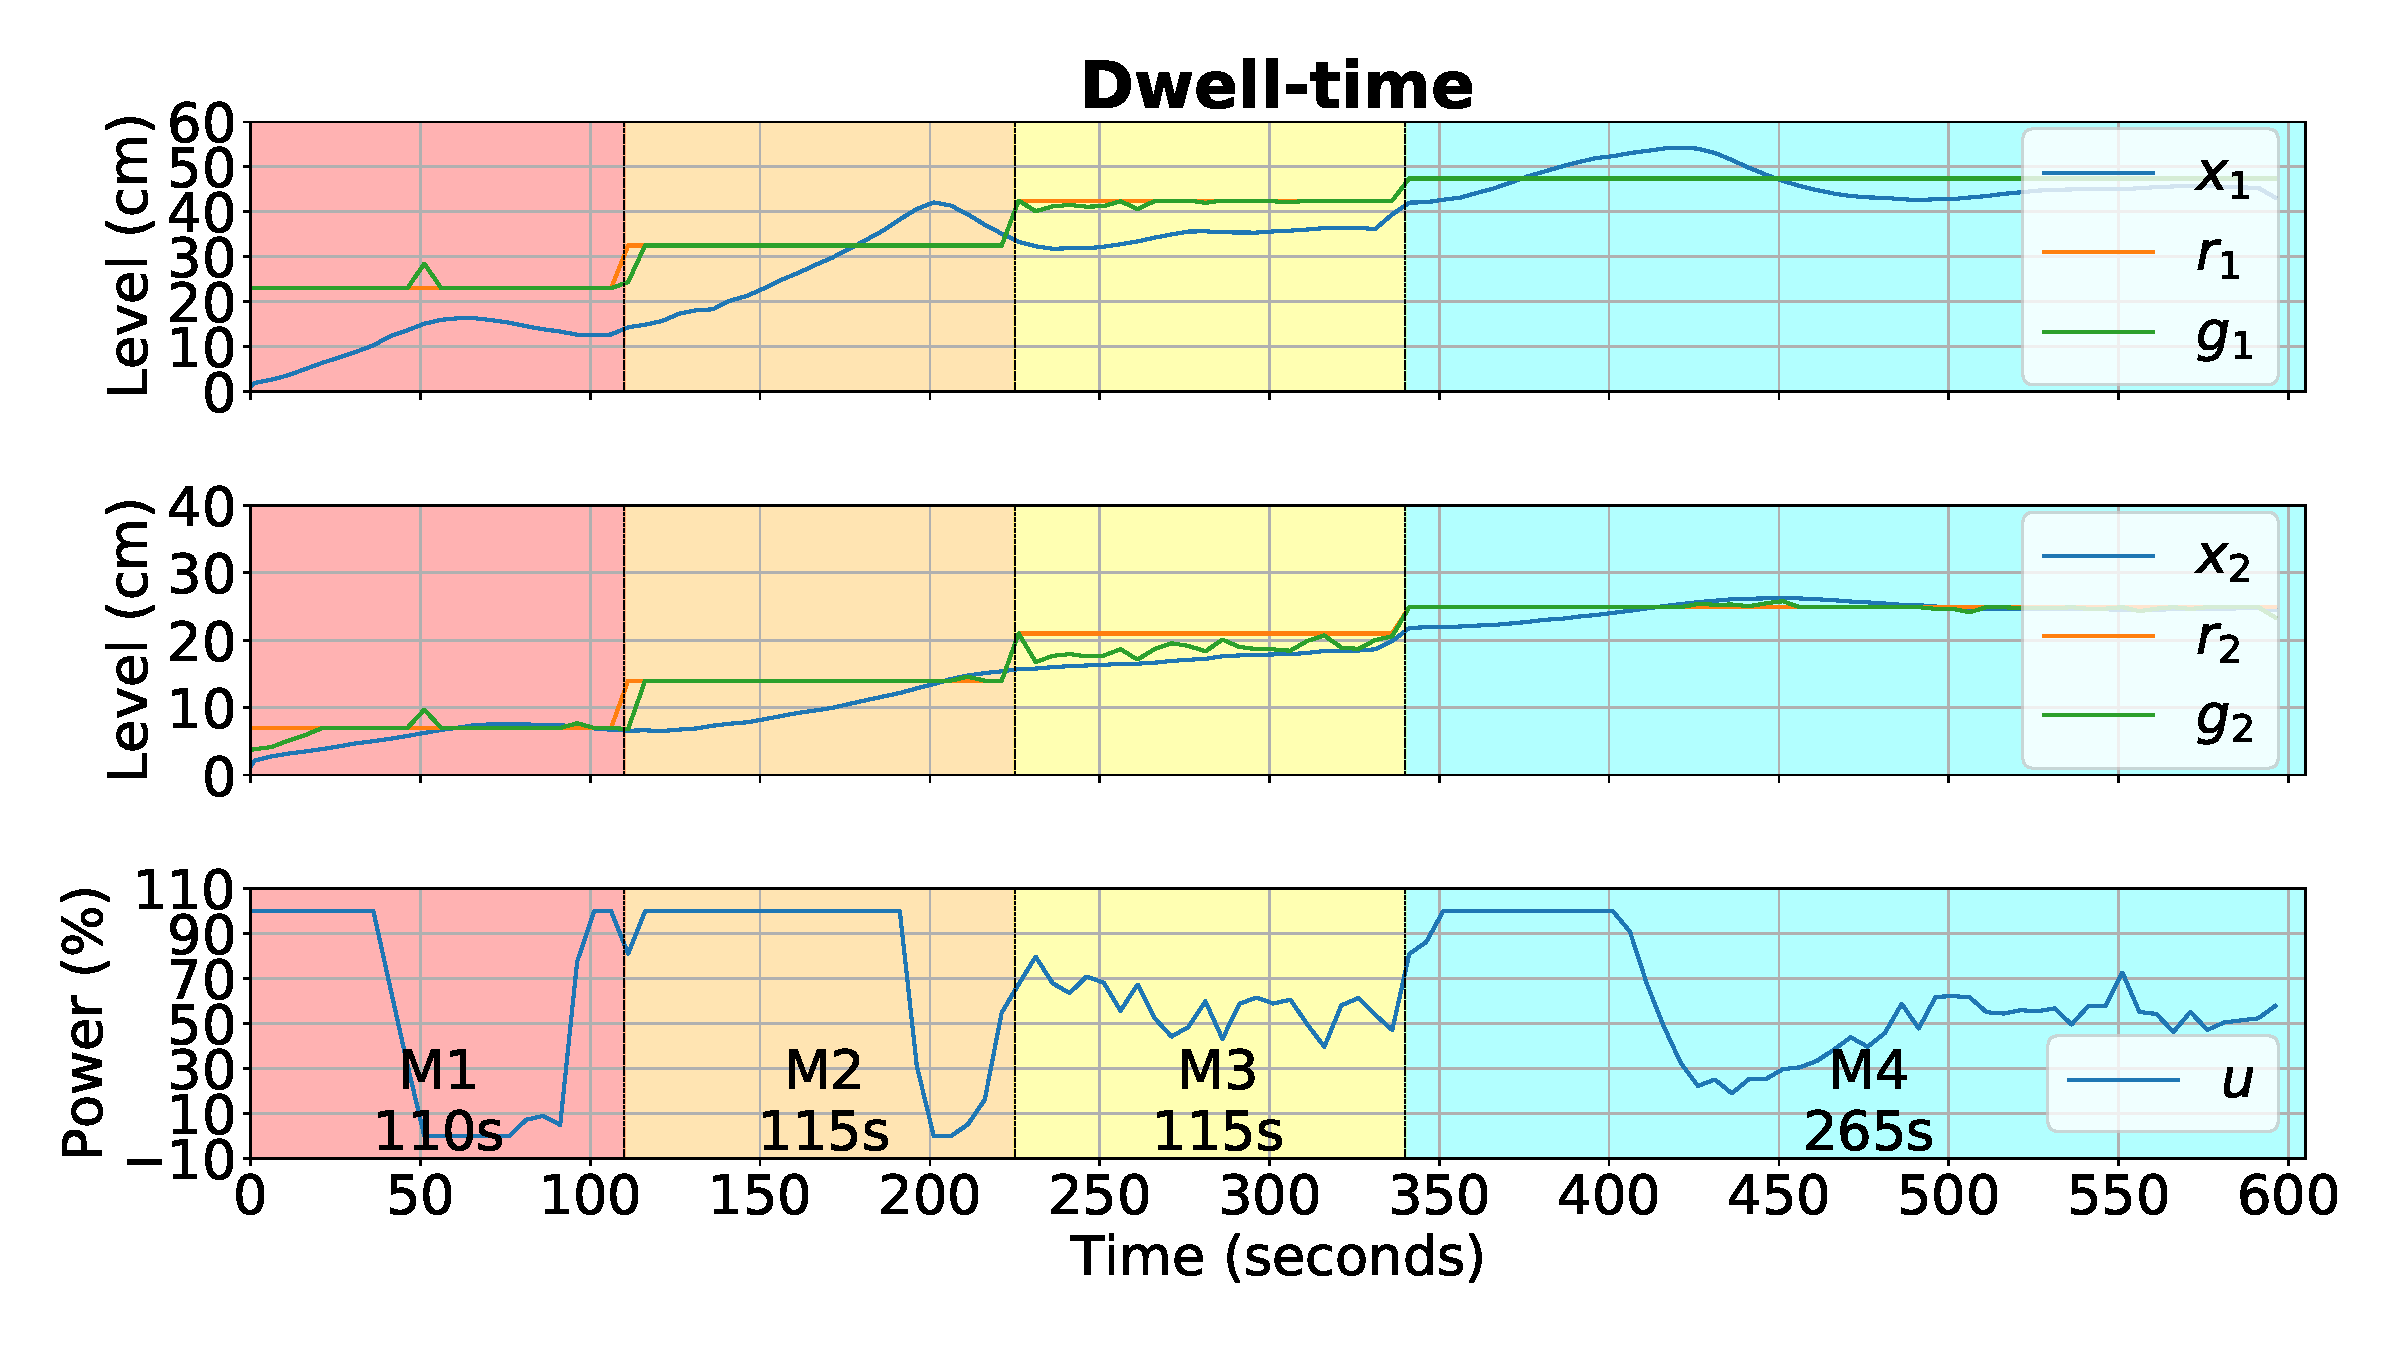
\includegraphics[width=\linewidth]{imgs/tanks-dwell}
  \caption[Experimental dwell-time states.]{This Figure shows the states and
    control signal of the system running with the dwell-time rule. The first two
    plots show the system states as well as the reference set by the supervisor
    and command governors and the third plot shows the control signal. All plots
    have colored backgrounds displaying the active mode, and the last plot also
    shows the time that each mode remained active. The states show overflows on
    first, second and fourth modes, which is expected from the system, and the
    control signal saturates four times and presents a large variation, going
    from 100\% to 0\%.}%
  \label{fig:tanks-dwell}
\end{figure}

\begin{figure}[ht!]
  \centering
  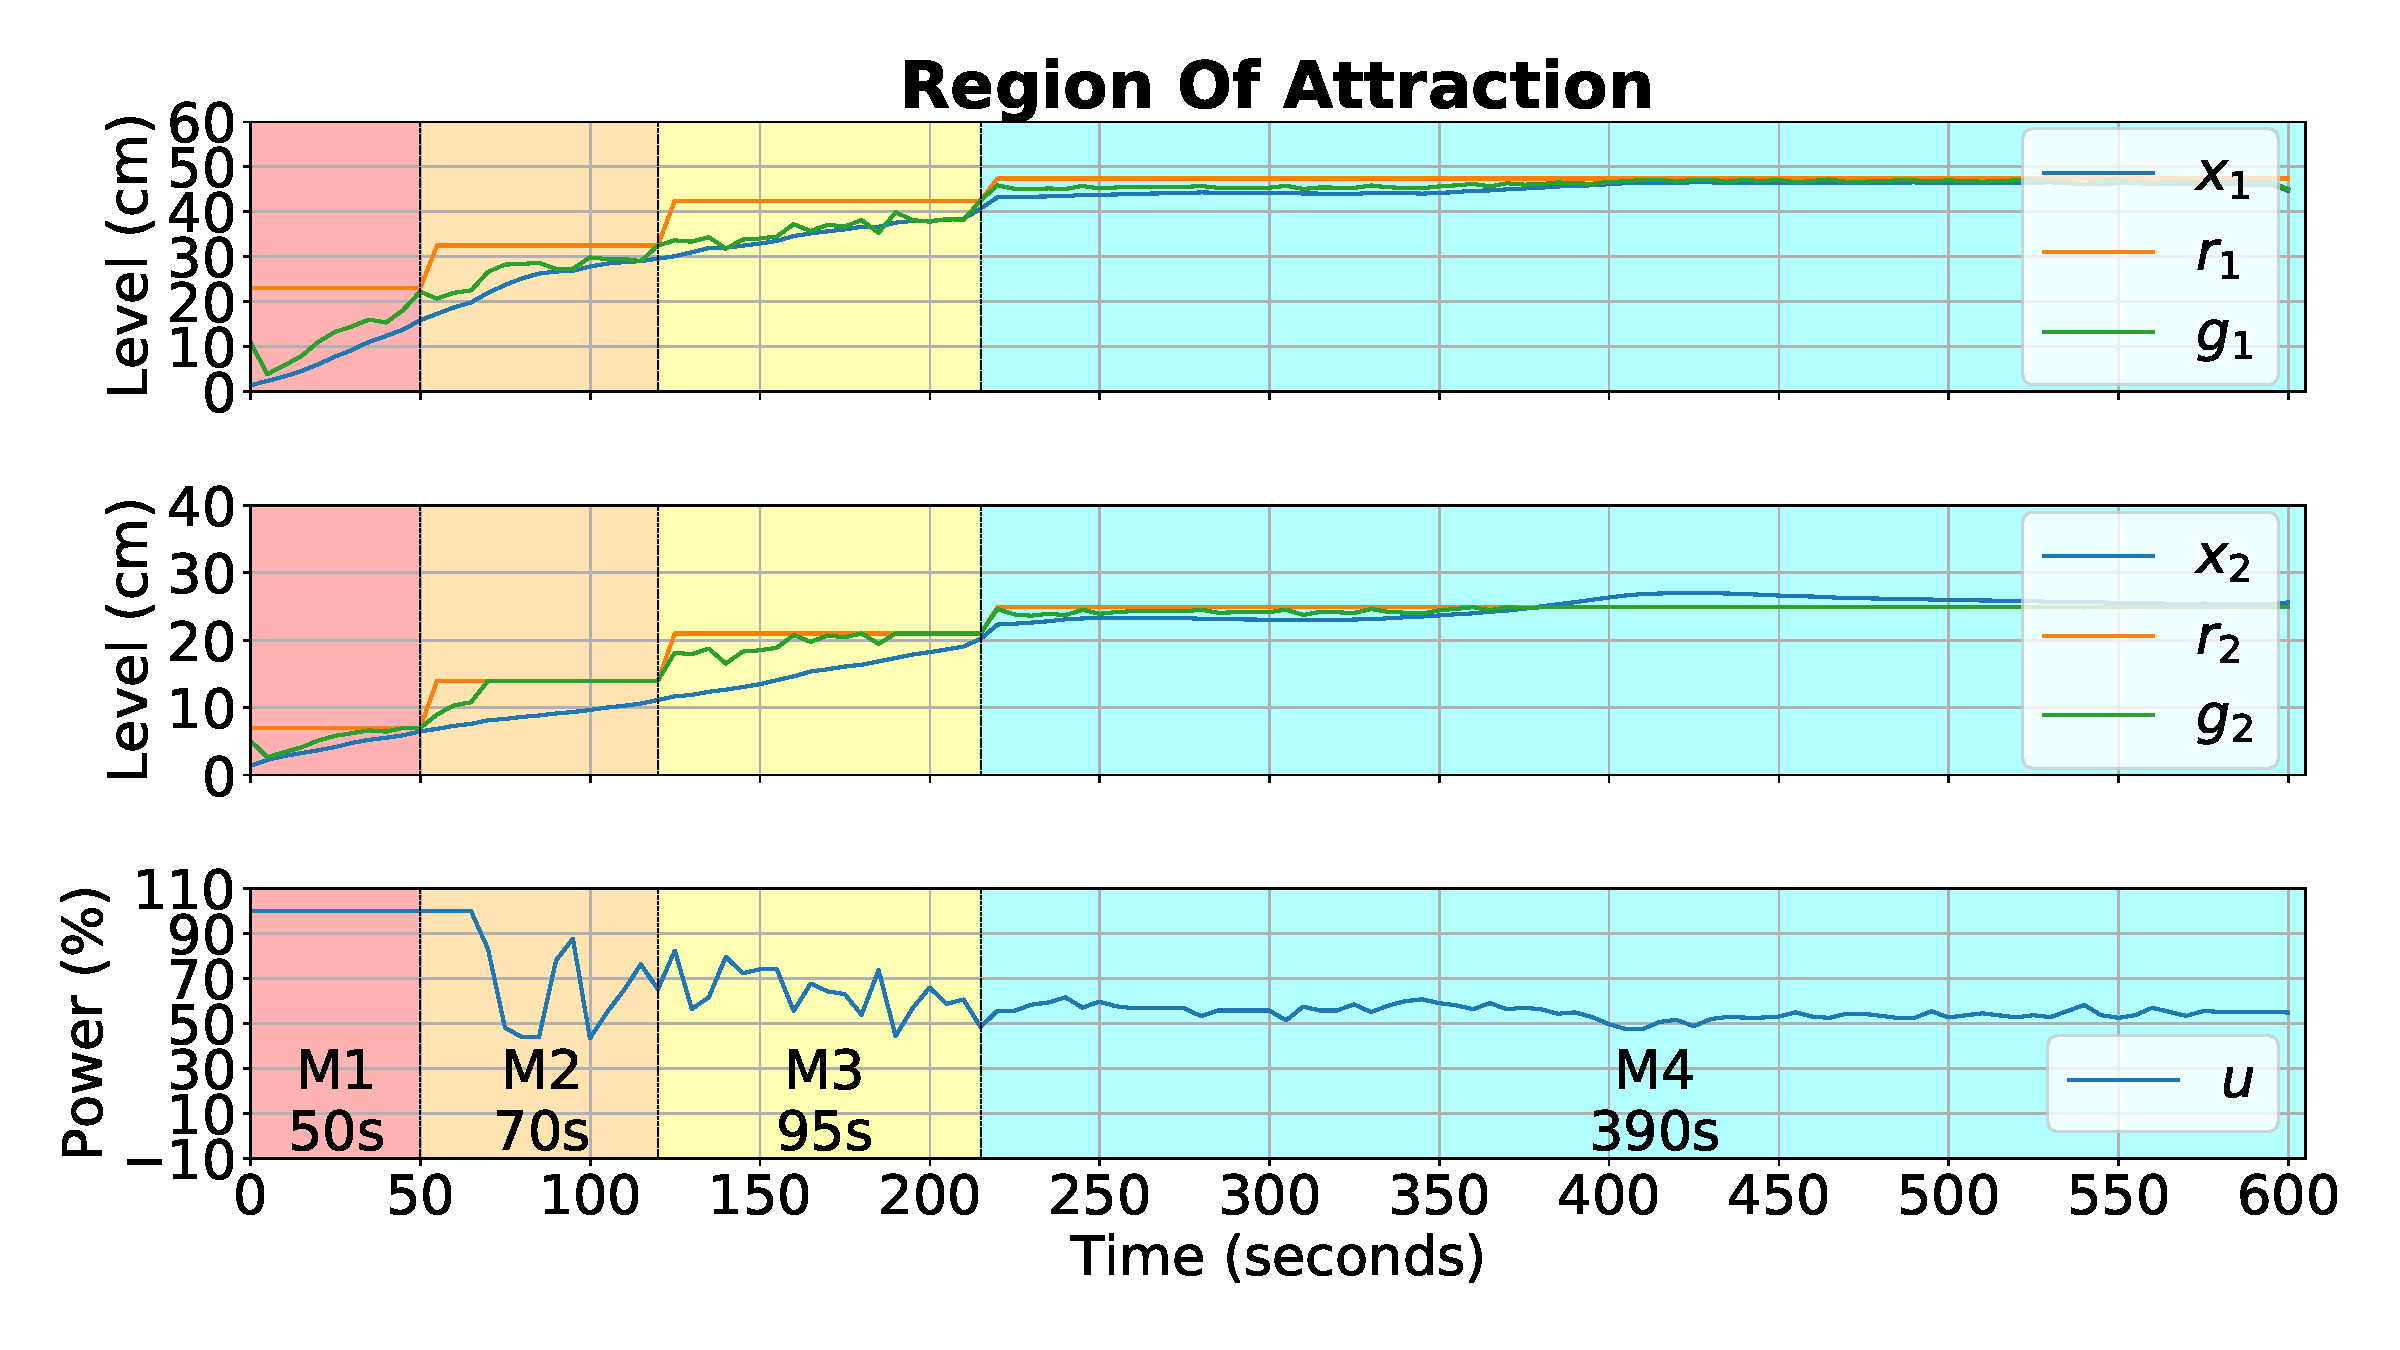
\includegraphics[width=\linewidth]{imgs/tanks-roa}
  \caption[Experimental RoA states.]{This Figure show the states and control
    signals of the Region of Attraction-based switching rule. It has the same
    structure as Figure~\ref{fig:tanks-dwell}. The overall convergence is
    visibly faster than the dwell-time alternative. Also, the states do not
    present overshoots, since the system is not given enough time to converge to
    the waypoints. The control signal has a smaler variation in amplitude only
    saturates at the begining.}%
  \label{fig:tanks-roa}
\end{figure}
